\documentclass[a4paper,12pt,twoside,hidelinks,openany]{report}

\usepackage[spanish]{babel}
\usepackage[utf8]{inputenc}
\usepackage[usenames, dvipsnames]{color}
\usepackage{graphicx}
\usepackage{enumerate}
\usepackage{multirow}
\usepackage{graphics}
\usepackage{appendix}
\usepackage[nottoc,numbib]{tocbibind}
\usepackage{float}

\usepackage{tikz}
\usetikzlibrary{shapes,arrows}
\usepackage{subcaption}
\usepackage{amsmath,amsthm,amssymb,mathrsfs}
\usepackage[final]{pdfpages}
\usepackage[]{placeins,flafter}
\usepackage[none]{hyphenat} \sloppy
\usepackage{xcolor}
\usepackage{adjustbox}

%	CONFIGURACIÓN DE PÁGINA

\setlength{\paperwidth}{21cm}          % Ancho de página
\setlength{\paperheight}{29,7cm}       % Alto de página
\setlength{\textwidth}{15.5cm}         % Ancho de zona con texto
\setlength{\textheight}{24.6cm}        % Ancho de zona con texto
\setlength{\topmargin}{-1.0cm}         % Margen superior

\setlength{\oddsidemargin}{0.46cm}     % Margen izquierdo
\setlength{\evensidemargin}{0.46cm}

\usepackage{makeidx}
\makeindex
\index{key}
\newcommand{\myref}[1]{\color{red}\bf(\ref{#1})}

\begin{document}

%%%%%%%%%%%%%%%%%%%%%%%%%%%%%%%%%%%%%%%%%%%%%%%%%%%%%%%%%%%%%%%%%%%%%%%%%%%%%%%%%%
%		PORTADA
%%%%%%%%%%%%%%%%%%%%%%%%%%%%%%%%%%%%%%%%%%%%%%%%%%%%%%%%%%%%%%%%%%%%%%%%%%%%%%%%%%

\begin{titlepage}

\vspace*{-4mm}
\begin{figure}[!h]
  \centering
	
\includegraphics[width=69.62mm]{Imagenes/UnizarLogo}
\end{figure}

\vspace*{17mm}

\fontsize{28pt}{28pt}\selectfont
\begin{center}
\setlength{\fboxsep}{3.4mm}
\adjustbox{minipage=14.4cm,cfbox=blue,center}{\begin{center} Trabajo Fin de Grado \end{center}}
\end{center}

\vspace*{18.7mm}


\fontsize{20pt}{20pt}\selectfont
\begin{center}
Diseño y análisis de redes homeostáticas adaptativas
\end{center}
\baselineskip 20pt
\begin{center}
Design and analysis of homeostatic adaptative networks
\end{center}

\vspace*{0cm}
\baselineskip 36pt
\begin{center}
\fontsize{12pt}{12pt}\selectfont
\center{\rm  Autor}

\vspace*{3.65mm}
\fontsize{18pt}{18pt}\selectfont
\center{Alberto Martínez Menéndez}
\vspace*{1cm}
\baselineskip 36pt
\fontsize{12pt}{12pt}\selectfont
\center{\rm  Directores}
\vspace*{3.56mm}
\fontsize{14pt}{14pt}\selectfont
\center{Manuel Gonzalez Bedía}
\end{center}

\setcounter{footnote}{1}

\vspace*{16.45mm}
\fontsize{12pt}{12pt}\selectfont
\begin{center}
ESCUELA DE INGENIERÍA Y ARQUITECTURA\\
2018\\
\end{center}


\renewcommand{\thefootnote}{\arabic{footnote}}
\pagenumbering{gobble}
\end{titlepage}
\newpage


\title{Diseño y análisis de redes homeostáticas adaptativas}
\author{Alberto Martínez Menéndez}

\pagebreak
\cleardoublepage
\baselineskip 19pt

\renewcommand{\labelitemi}{$-$}
\renewcommand{\tablename}{Tabla}

\renewcommand{\appendixname}{Anexos}
\renewcommand{\appendixtocname}{Anexos}
\renewcommand{\appendixpagename}{Anexos}


\pagenumbering{Roman}

%%%%%%%%%%%%%%%%%%%%%%%%%%%%%%%%%%%%%%%%%%%%%%%%%%%%%%%%%%%%%%%%%%%%%%%%%%%%%%%%%%%
%		Declaración de autoría y originalidad
%%%%%%%%%%%%%%%%%%%%%%%%%%%%%%%%%%%%%%%%%%%%%%%%%%%%%%%%%%%%%%%%%%%%%%%%%%%%%%%%%%%

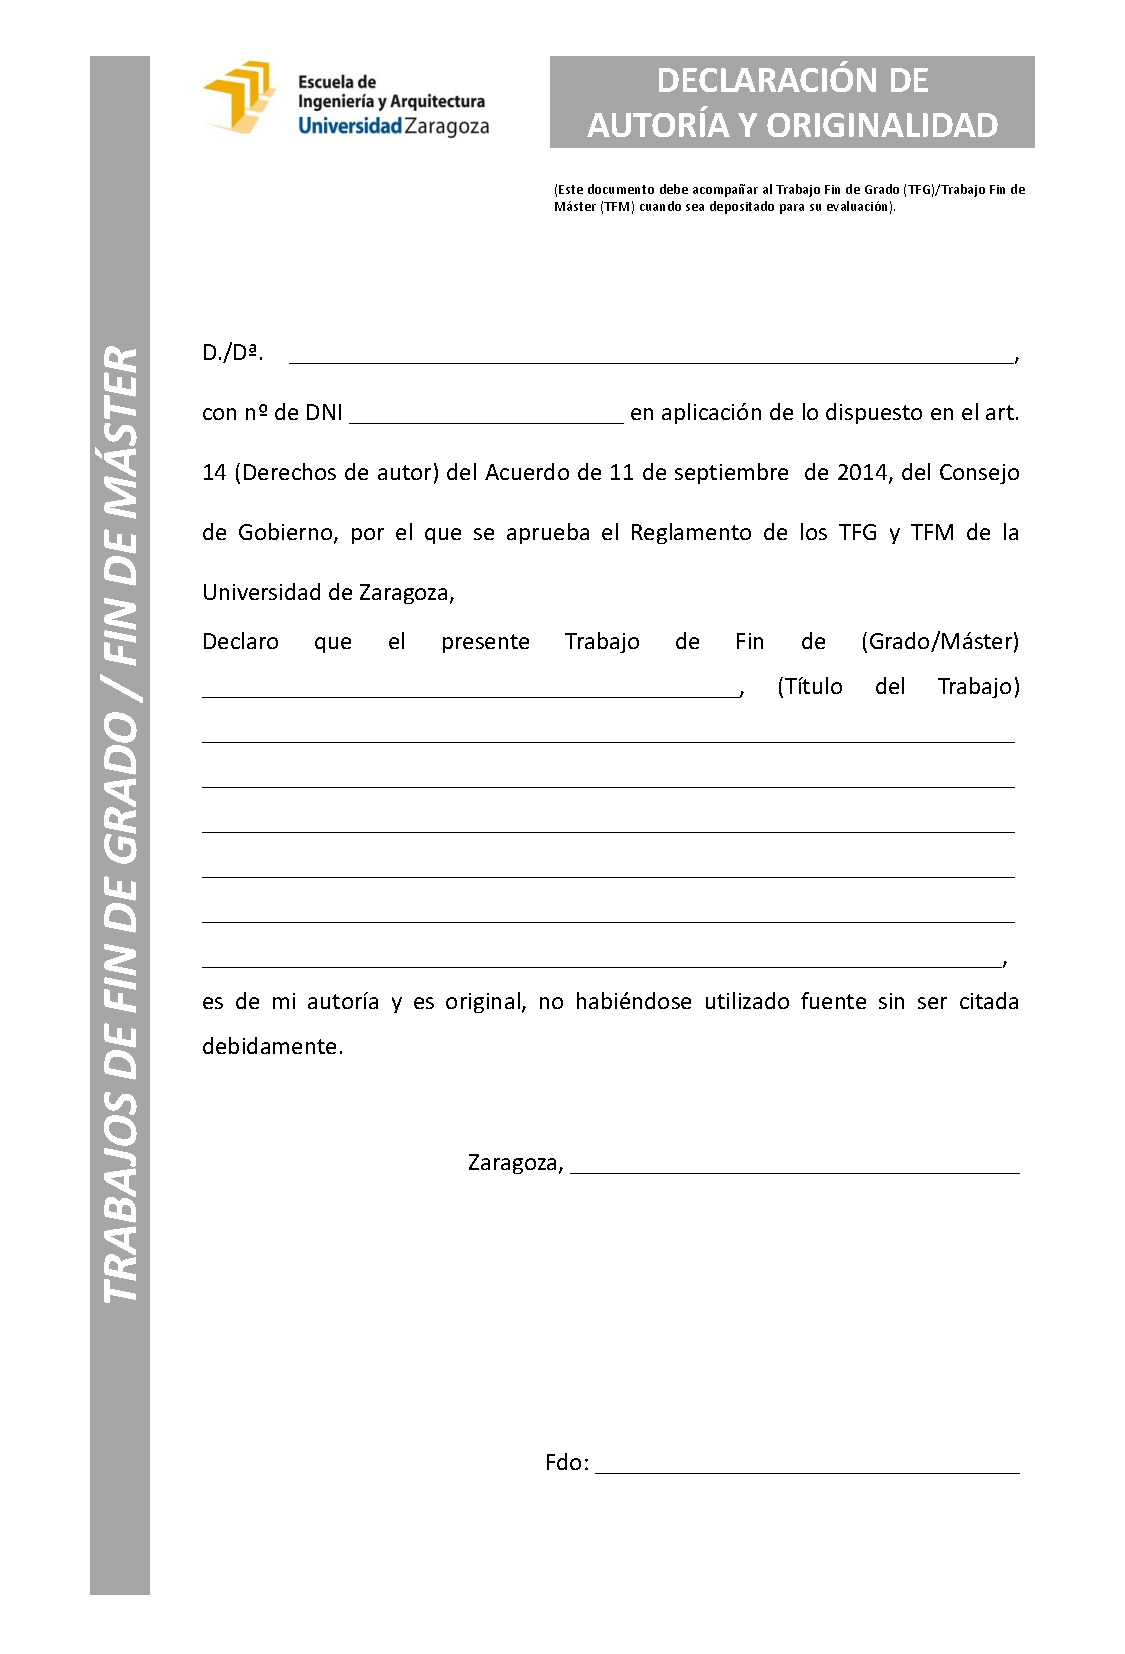
\includepdf[pagecommand={}]{Impresos/Autoria}
\cleardoublepage

%%%%%%%%%%%%%%%%%%%%%%%%%%%%%%%%%%%%%%%%%%%%%%%%%%%%%%%%%%%%%%%%%%%%%%%%%%%%%%%%%%%
%		Resumen
%%%%%%%%%%%%%%%%%%%%%%%%%%%%%%%%%%%%%%%%%%%%%%%%%%%%%%%%%%%%%%%%%%%%%%%%%%%%%%%%%%%

\newpage

\newpage
\cleardoublepage
\begin{center}
{\Large \bfseries Diseño y análisis de redes homeostáticas adaptativas}

\vspace{1cm}
{\Large \bfseries RESUMEN}

\vspace{1.5cm}
\end{center}

Conseguir dotar a un agente artificial con la capacidad de adaptabilidad presente en los seres vivos le proporcionaría habilidades necesarias para realizar tareas para las que no ha sido entrenado o
para las que se le ha entrenado pero en un entorno cambiante o con incertidumbre. En este trabajo nos interesaremos, desde una perspectiva ingenieril, por unos de los sistemas de autoregulación presentes
en los organismos vivos conocidos como mecanismos homeostáticos, que están en la base de ciertas capacidades de adaptación.

En particular, se ha partido del diseño e implementación de un agente homeostático basado en redes neuronales recurrentes de tiempo continuo con capacidad de fototaxis (búsqueda y acercamiento a una serie de luces en un espacio).
Este agente se corresponde con el mejor candidato de una cierta población, seleccionado mediante un algorítmo genético. La peculiaridad del mismo, es que despliega comportamiento homeostático a través de mecanismos de plasticidad,
que le permiten modificar sus variables internas para alcanzar un estado estable y mantenerse en el mismo aunque se vea sometido a perturbaciones externas.

Una vez obtenido el agente con las propiedades de fototaxis y plasticidad homeostática, se ha buscado dotar al mismo de capacidades para que emerjan comportamientos sociales con el fin de analizar cómo interacciona en situaciones donde hay más de un agente
involucrado. El comportamiento social se ha añadido siguiendo dos aproximaciones diferentes. La primera, asume que las capacidades del agente son aditivas. Es decir, que el agente tras ser capaz de navegar y orientarse
hacia un foco de luz (o comida), necesitaría una nueva estructura neuronal con la que codificar otra capacidad novedosa (en este caso, coordinación social). Se modelará el sistema con dos mecanismos independientes en el controlador
del sistema, uno para la navegación y otro para el aspecto social. La segunda, defiende que el comportamiento social es una característica estructural del sistema. Por tanto, una nueva capacidad atraviesa (en ocasiones se
dice que ``percola'') las capacidades previas, reestructurando el controlador neuronal del agente en su conjunto. El objetivo es comparar estas dos aproximaciones y sacar conclusiones sobre ello mediante experimentos en los que
varios agentes tienen que interactuar de manera social para la consecución de un objetivo.

\newpage
\begin{center}
{\Large \bfseries Design and analysis of homeostatic adaptative networks}

\vspace{1cm}
{\Large \bfseries ABSTRACT}

\vspace{2.5cm}
\end{center}


El resumen pero traducido al ingles


\cleardoublepage
\renewcommand{\contentsname}{Índice}
\tableofcontents

%%%%%%%%%%%%%%%%%%%%%%%%%%%%%%%%%%%%%%%%%%%%%%%%%%%%%%%%%%%%%%%%%%%%%%%%%%%%%%%%%%%
%		Listas de figuras y tablas
%%%%%%%%%%%%%%%%%%%%%%%%%%%%%%%%%%%%%%%%%%%%%%%%%%%%%%%%%%%%%%%%%%%%%%%%%%%%%%%%%%%
\newpage
\renewcommand\listfigurename{Lista de Figuras}
\listoffigures

\newpage
\renewcommand\listtablename{Lista de Tablas}
\listoftables

%%%%%%%%%%%%%%%%%%%%%%%%%%%%%%%%%%%%%%%%%%%%%%%%%%%%%%%%%%%%%%%%%%%%%%%%%%%%%%%%%%%
%		Capitulos
%%%%%%%%%%%%%%%%%%%%%%%%%%%%%%%%%%%%%%%%%%%%%%%%%%%%%%%%%%%%%%%%%%%%%%%%%%%%%%%%%%%

\chapter{Introducción}
\pagenumbering{arabic}
Incorporar comportamiento adaptativo en agentes artificales es uno de los medios esenciales para que estos puedan desenvolverse en entornos con cambios o incertidumbre de manera satisfactoria.

En ingeniería, uno de los pioneros trabajos en este ámbito se debe a William Ashby ('A Design for a Brain'), en el que se interesó por investigar como funcionan los mecanismos de
adaptación en sistemas vivos. La tesis de Ashby fue que todos los organismos tienen ciertas variables esenciales, que deben mantenerse dentro de unos límites, y que a menudo están
vinculadas entre sí, provocando que cambios en algunas de ellas puedan afectar a las demás. El estado de supervivencia del organismo ocurre cuando un comportamiento no mueve ninguna variable esencial
fuera de sus límites. Al conjunto de mecanismos que permiten esta estabilidad se lo conoce como regulación homeostática. En lugar de atribuir a los organismos conductas intencionales de búsqueda de objetivos,
Ashby exploró estos mecanismos que permitían generar un comportamiento adaptativo autoinducido mediante el mantenimiento de la estabilidad interna de sus variables esenciales.

Trabajos recientes en neurociencia han mostrado que existen mecanismos reguladores homeostáticos de eficacia sináptica en el cerebro. Estos mecanismos entre neuronas están impulsados por la
necesidad de adaptarse a los cambios que dependen de una actividad, al tiempo que mantienen la estabilidad interna.

Dotar a un agente artificial de propiedades de adaptación homeostática le permitiría adaptarse y resolver problemas para los que inicialmente no fue entrenado, permitiéndole alterar sus variables
internas hasta obtener una estabilidad completa de su sistema al mismo tiempo que ejecuta las tareas encomendadas.

\section{Contexto y motivación}
Me planteo estudiar el comportamiento..... para ...... TODO TODO TODO

\section{Objetivos}
En este trabajo de fin de grado se pretenden aplicar y analizar las ideas de
ultrastabilidad de William Ashby en agentes artificiales. Dichos agentes serán diseñados mediante controladores
basados en redes neuronales recurrentes a las que se les impondrá una regulación
homeostática de su actividad sináptica (las neuronas tendrán funciones de activación
adecuadas para generar estas estructuras de estabilidad). Los agentes serán evolucionados
para solucionar un problema de fototaxis (búsqueda y acercamiento a una fuente de luz).
Una vez programados agentes artificiales homeostáticos se buscará analizar:

\begin{itemize}
\item Si los agentes pueden adaptarse a cambios en las reglas del entorno, aunque no hayan
evolucionado específicamente para resolver nuevas tareas. Se buscará probar que, tal
como ocurre en organismos vivos, estos mecanismos de adaptación facilitan
implícitamente el mantenimiento de estabilidad y el desarrollo de nuevos
comportamientos.
\item  Si en entornos sociales de agentes artificiales, donde los comportamientos para resolver
problemas se basen en estrategias colectivas, los patrones de estabilidad son más
robustos. Para ello se someterán las configuraciones obtenidas a estímulos ruidosos o
perturbaciones, y mediremos el grado de estabilidad de los patrones homeostáticos.
\end{itemize}

\section{Estructura}
La memoria cuenta con un primer apartado de introducción, seguido por otro del estado del arte, en los que se explica el contexto del problema a resolver, los principales objetivos,
motivaciones y situación actual del ámbito en el que se desarrolla el trabajo. A continuación se encuentra el apartado de diseño e implementación, en el cual se habla sobre las distintas
herramientas y técnicas utilizadas para la realización del trabajo. Por último, en la sección de experimentación se enuncian y se analizan los dos procesos que se han ejecutado para la
realización de los dos objetivos anteriormente descritos.

En los anexos se puede observar el tiempo invertido en este proyecto junto con las tareas las que se dedicó. Además,
se incluye el código correspondiente en el lenguaje de programación Python desarollado para la obtención de los resultados necesarios.

\chapter{Estado del arte}
\pagenumbering{arabic}
TODO TODO TODO Hablar description
HABITOS (frente a comportamientos programados)
CTRNNs (capacidad de representar cualquier modelo e incluso de actuar como memoria para otras neuronas)
Regla de Hebb (Relacionar homeostasis con la regla de Hebb)
Ultraestabilidad de Ashby

\chapter{Fundamentos teóricos}
\pagenumbering{arabic}

\section{Redes neuronales recurrentes de tiempo continuo (CTRNN)}
En contraste con las redes neuronales feed-forward, las cuales soportan únicamente comportamientos
reactivos, en las Redes Neuronales Recurrentes de Tiempo Continuo (CTRNN) \cite{BeerRD}
pueden existir ciclos en su estructura y la activación de sus neuronas es asíncrona y multiescalada
en el tiempo. Este tipo de redes neuronales también facilita describir el agente como un
sistema dinámico acoplado al entorno en el que está ubicado, ya que está demostrado que son el
modelo más simple de red neuronal dinámica continua no lineal \cite{FunaYNaka}
Además, la interpretación neurobiológica de las CTRNN ha sido demostrada y puede consultarse
en \cite{BeerRD}.

\subsubsection{Descripción matemática de una CTRNN}
Las CTRNN están formadas por neuronas cuyo comportamiento se describe en las ecuaciones \ref{eq:funcionCTRNN} y \ref{eq:funcionSIGMOIDE}
\begin{equation} \label{eq:funcionCTRNN}
	\dot{y_{i}}= \frac{1}{\tau_{i}} * \left ( -y_{i}+\sum_{j=1}^{N}w_{ji}*\sigma \left ( y_{j} + \theta _{j} \right ) + I_{i} \right ) \qquad i =1,2,...,N
\end{equation}
\begin{equation} \label{eq:funcionSIGMOIDE}
	\sigma (x)=\frac{1}{1+e^{-x}}
\end{equation}
donde $y_{i}$ es el estado de la neurona, $w_{ji}$ es el peso de la conexión entre las neuronas i y j,
$\theta$ es el término bias, I representa una entrada externa y $\tau$ hace que cada una de las neuronas
dependa del tiempo, ya que para diferentes valores la caída del nivel de activación de la neurona
es más rápida o lenta. En la fórmula \ref{eq:funcionCTRNN} la velocidad de actualización de la red neuronal debe ser
notablemente mayor (el intervalo entre dos actualizaciones será menor) que el valor de $\tau$ para no
obtener comportamientos no deseados.

\subsubsection{Valores de activación y de salida de la neurona de una CTRNN}
Para poder entender cómo deben interpretarse la activación y la salida de una CTRNN, se va
a utilizar como ejemplo una CTRNN formada por una única neurona autoconectada como la de la figura \ref{fig:figuraCTRNNBasica}.
El valor de salida o de una neurona será un valor real entre 0 y 1 obtenido al aplicar la función
sigmoide (ecuación \ref{eq:funcionSIGMOIDE}) a la suma del estado actual y de la neurona con su valor bias $\theta$, tal y
como puede verse en la figura \ref{fig:figuraCTRNNBasica}.
\begin{figure}[H]
    \centering
    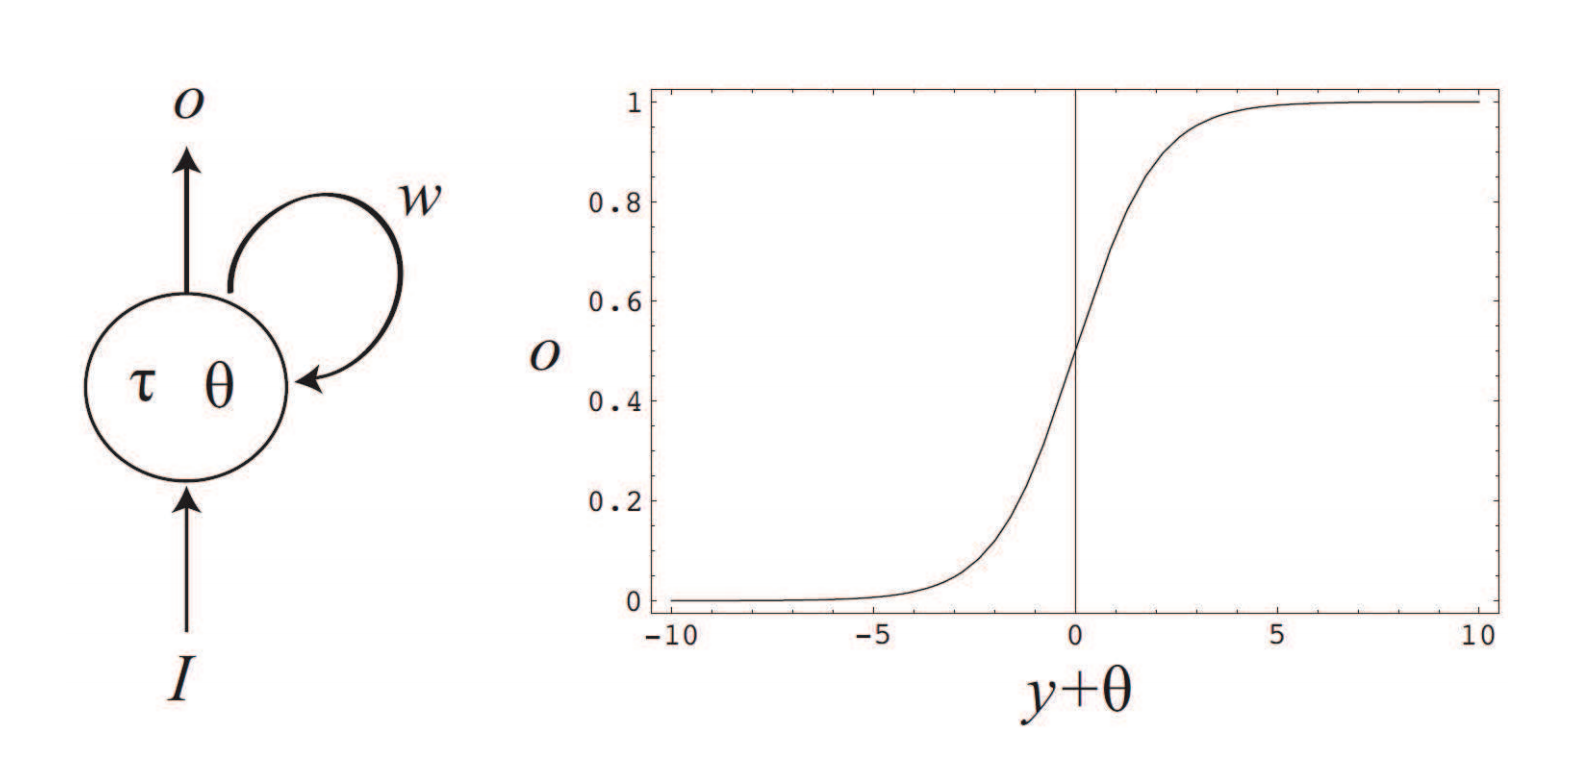
\includegraphics[width=0.8\textwidth,height=6cm]{Imagenes/CTRNNBasica}
    \caption{Valor de salida de una CTRNN. \textbf{Izquierda:} Un nodo autoconectado. \textbf{Derecha:} Función sigmoide aplicada para calcular la salida de una neurona.}
    \label{fig:figuraCTRNNBasica}
\end{figure}

En cuanto al valor de activación, a diferencia de una red neuronal feed-forward, la cual realiza
un mapeo directo entre entrada y salida de la red, el comportamiento de una CTRNN corresponde
al de un sistema dinámico \cite{BeerRD}, por lo que el valor de activación de la neurona convergerá
a un punto de equilibrio. Para el análisis de las dinámicas del sistema formado por el agente
controlado por la CTRNN y el entorno, se analizarán sus diagramas de bifurcación, los cuales
muestran todos los puntos de equilibrio para la activación de las neuronas de la red.

\section{Homeostasis}
A pesar de que la homeostasis es una propiedad biológica, es posible representar un sistema lógico que se comporte de forma similar a como
sistemas vivos con estas propiedades lo harían\cite{Hywel}.

Un \textit{Homeostato}, es un sistema artificial que presenta porpiedades de homeostasis. El Homeostato desarrollado por Ashby era un aparato
electromagnético mientras que el que va a ser utilizado es un componente implementado computacionalmente.

Un Homeostato es un sistema de $N$ neuronas completamente interconectadas entre si. Cada neurona recibe $N$ entradas, de si misma y del resto de neuronas,
dependientes del peso de la fuerza de conexión de las uniones entre ellas (ver Figura \ref{fig:figuraHomeostatSchema}).

\begin{figure}[!h]
    \centering
    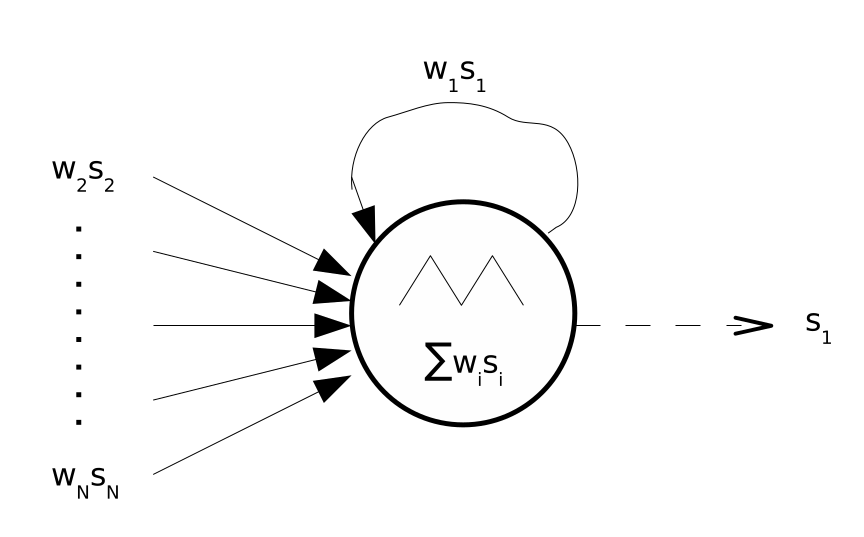
\includegraphics[width=0.6\textwidth,height=5cm]{Imagenes/HomeostatSchema}
    \caption{Esquema de un Homeostato individual. La unidad recibe las entradas del resto de unidades ($w_{i}s_{i}$) y de si misma ($w_{1}s_{1}$). La salida $s_{1}$ es una función lineal por partes
		de la suma ponderada de las entradas.)}
    \label{fig:figuraHomeostatSchema}
\end{figure}

\begin{figure}[!h]
    \centering
    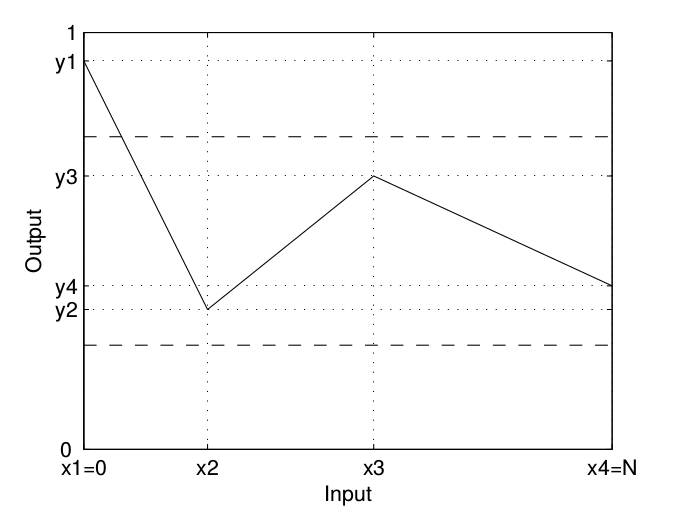
\includegraphics[width=0.6\textwidth,height=6cm]{Imagenes/HomeostatTransfer}
    \caption{Ejemplo de función de transferencia de una unidad Homeostat. La función es lineal por partes con puntos en ($x_{1},j_{1}$),...,($x_{p},y_{p}$) donde $x_{1}$ = 0 y $x_{p}$ = $N$, para todas las
		unidades en una red de $N$ unidades. Las líneas discontinuas representan el rango homeostatico de la red.}
    \label{fig:homeostatTransferFunction}
\end{figure}

La suma ponderada $I$ (ver ecuación \ref{eq:sumaPonderadaHomeostat}) de las entradas de una unidad determina su salida $s$, tal y como está especificado por la función linear de transferencia por
partes $F$ (ecuación \ref{eq:ecuPartesHomeostat} y figura \ref{fig:homeostatTransferFunction}).

\begin{equation} \label{eq:sumaPonderadaHomeostat}
	I = \sum_{i}^{N}w_{i}s_{i}
\end{equation}

\begin{equation} \label{eq:ecuPartesHomeostat}
	s = F(I)=\begin{cases}
y_{1}+(y_{2}-y_{1})(\frac{I-x_{1}}{x_{2}-x_{1}}) & \text{ : }\quad x_{1} \leq I < x_{2} \\
y_{2}+(y_{3}-y_{2})(\frac{I-x_{2}}{x_{3}-x_{2}}) & \text{ : }\quad x_{2} \leq I < x_{3} \\
y_{3}+(y_{4}-y_{3})(\frac{I-x_{3}}{x_{4}-x_{3}}) & \text{ : }\quad x_{3} \leq I \leq  x_{4} \\
\end{cases}
\end{equation}

Al inicializar la red, los pesos de las conexiones se aleatorizan a partir de una distribución uniforme de rango apropiado. El rango objetivo (o rango límite) $R = [0.5 - \delta, 0.5 + \delta]$ es
especificado para la salida, donde $\delta$ determina la rigidez de la restricción homeostática. Si $s \in R$ la unidad es homeostática. Si $s \notin R$ significa que la homeostasis se ha perdido
y se activan los mecanismos de cambio adaptativo.

Hay dos mecanismos de cambio adaptativo que se aplican a los parámetros de las unidades no homeostáticas. El primer mecanismo asigna valores aleatorios a los pesos de las conexiones aferentes a la unidad (ecuación \ref{eq:aferenteEQ}).
El segundo mecanismo asigna nuevos valores aleatorios a los parámetros que indican las coordenadas de la función de transferencia de la unidad (ecuación \ref{eq:transferEQ}). Los rangos de estas reasignaciones son los mismos utilizados
en la inicialización. Donde $rand(a,b)$ representa a la función que devuelve un número real aleatorio obtenido de una distribución uniforme en el rango $[a,b]$.

\begin{equation} \label{eq:aferenteEQ}
	\text{\textit{IF}} \quad (s \notin R) \quad \text{\textit{THEN}} \quad [w= \text{\textit{rand}}(0.00, 1.00) \quad \forall w \in \left \{ w_{1},...,w_{N} \right \}]
\end{equation}

\begin{equation} \label{eq:transferEQ}
	\begin{aligned}
	 \text{\textit{IF}} \quad (s \notin R) \quad \text{\textit{THEN}} \quad [x= \text{\textit{rand}}(0.00, N) \quad \forall x \in \left \{ x_{2},...,x_{p-1} \right \}]& \\
	 \qquad \qquad \qquad \,\quad  \text{\textit{AND}} \quad [y= \text{\textit{rand}}(0.00, 1.00) \quad \forall y \in \left \{ y_{1},...,y_{p} \right \}]& \\
 \end{aligned}
\end{equation}

Durante la realización de este trabajo de diseñó e implementó un sencillo Homeostato para comprender mejor los fundamentos que lo definen. La descripción de este Homeostato puede encontrase en el Anexo \ref{ch:anexo1} y puede servir como
ejemplo sencillo para ayudar a comprender los fundamentos de la homeostasis.


\section{Algoritmo genético}
Los algoritmos genéticos son un método para resolver problemas de optimización. Estos algoritmos están basados en la selección natural, que es el proceso que dirige la evolución biológica. Un algoritmo genético modifica repetidas veces
una poblacion de posibles soluciones. En cada iteración, se seleccionan las mejores posibles soluciones encontradas hasta el momento y se genera a partir de ellas una nueva generación de candidatos. Generación tras generación la
población evoluciona hacia la solución óptima.

Los algoritmos genéticos difieren de los los algoritmos clásicos de optimización en tres puntos principales:
\begin{enumerate}
	\item{Los algoritmos clásicos generan un único punto con cada iteración mientras que los algoritmos genéticos generan una población de puntos con cada iteración.}
	\item{En los algoritmos clásicos la secuencia de puntos se aproxima en cada iteración a la solución óptima mientras que en los algoritmos genéticos es el mejor punto de la población el que se aproxima a la solución óptima.}
	\item{Los algoritmos clásicos generan el siguiente punto de la secuencia mediante un cálculo determinista mientras que los algoritmos genéticos selecciona el siguiente punto en la secuencia mediante cálculos que utiliza generadores de números aleatorios.}
\end{enumerate}

Una descripción más detalla de los algoritmos genéticos, tanto de su funcionamiento como de las partes que lo componen, puede encontrarse en el Anexo \ref{ch:anexo2}.

\chapter{Modelo e implementación}
\pagenumbering{arabic}
Para la realización de este trabajo, se han diseñado y desarrollado una serie de agentes a los que se les ha entrenado para la obtención de un comportamiento de fototaxis, es decir, de
búsqueda y acercamiento a fuentes de luz.

Cada agente está modelado como si tuviera un cuerpo esférico con dos sensores en la parte frontal que permiten recibir lecturas de los diferentes estímulos presentes (ya sean luces u otros agentes) y dos motores opuestos
que permiten que el agente pueda moverse libremente por el espacio, como puede verse
en la figura \ref{fig:figuraMyAgent}. El agente tiene en todo momento una posición en el espacio dada por unas coordenadas (x, y), así como una orientación respecto al eje X. Cada sensor está separado
60º del eje de orientación del agente. Los sensores tienen un arco de visión de 160º, para representar que el propio cuerpo del agente pueda encontrarse entre el sensor y la luz, evitando las lecturas.

\begin{figure}[H]
	\centering
	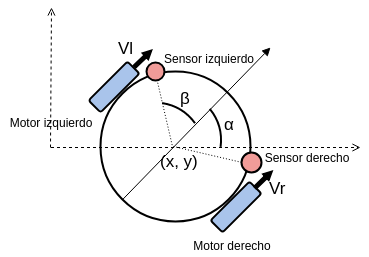
\includegraphics[width=0.6\textwidth,height=6cm]{Imagenes/Agent}
	\caption{Esquema del agente utilizado.}
	\label{fig:figuraMyAgent}
\end{figure}

El movimiento traslacional del agente se calcula a partir de la velocidad lineal ($v$) de su centro de masa (ecuación \ref{eq:VFormula}). El movimiento angular del agente se calcula obteniendo
la velocidad angular ($\omega$) de su centro de masa (ecuación \ref{eq:WFormula}).

\begin{equation} \label{eq:VFormula}
 \centering
 v = \frac{Vr + Vl}{2}
\end{equation}

\begin{equation} \label{eq:WFormula}
 \centering
 \omega = \frac{Vr - Vl}{2R}
\end{equation}

La nueva posición del agente para cada ciclo de ejecución se calcula mediante las ecuaciones (\ref{eq:newXformula}, \ref{eq:newYformula} y \ref{eq:newAformula}), donde $x$ e $y$ representan la posición actual del agente,
$\theta$ representa la orientación actual del agente y $\delta t$ representa el tamaño del tiempo de integración de ciclo.

\begin{equation} \label{eq:newXformula}
 \centering
 x(t + 1) = x(t) + v.cos(\theta).\delta t
\end{equation}

\begin{equation} \label{eq:newYformula}
 \centering
 y(t + 1) = y(t) + v.sin(\theta).\delta t
\end{equation}

\begin{equation} \label{eq:newAformula}
 \centering
 \delta (t + 1) = \delta (t) + \omega .\delta t
\end{equation}

Los sensores obtendran en cada iteración, si tienen visual directo con la luz, lecturas sobre la intensidad que perciben de ella. La intensidad($I$) que recibe cada sensor se calcula con la fórmula \ref{eq:intensity}, donde
la \textit{Intensidad de la fuente} es la intensidad que emite la fuente de luz y $D^{2}$ es la distancia entre el sensor que realiza la lectura y la fuente de luz.
\begin{equation} \label{eq:intensity}
 \centering
 I = \frac{\text{Intensidad de la fuente}}{D^{2}}
\end{equation}

Para los experimentos realizados en este trabajo, el radio del agente siempre se ha tomado como \textbf{4.0}.

\subsection{Plasticidad}
La ultraestabilidad de los agentes desarrollados se ha conseguido dotando a los mismos de mecanismos de plasticidad, que les permiten modificar los valores de algunos de sus atributos internos. En este caso, los agentes pueden
alterar los valores de los pesos $w_{ij}$ de las conexiones entre las neuronas de la red cuando la frecuencia de activación de una neurona es demasiado baja o demasiado alta.

La homeostasis no se encuentra programada explícitamente, pero aparece de forma implícita debido a los mecanismos de evaluación de la evolución genética que recompensan con mejor puntuación a aquellos
agentes que, durante la realización del entrenamiento, han mantenido un mayor número de sus neuronas estables.

La plasticidad de cada conexión está gobernada por la actividad sináptica de la conexión junto con una regla de plasticidad codificada genéticamente. Estas reglas de plasticidad vienen dadas por las
ecuaciones (\ref{eq:R0plasticityRule}, \ref{eq:R1plasticityRule}, \ref{eq:R2plasticityRule} y \ref{eq:R3plasticityRule}), donde $\Delta w_{ij}$ es el incremento por unidad de tiempo de un determinado peso sináptico ($w_{ij}$), y $z_{i}$ y $z_{j}$ son las frecuencias de
activación de las neuronas presinápticas y postsinápticas respectivamente.

Las reglas de plasticidad se construyen en torno a cuatro parámetros: la frecuencia de aprendizaje ($n_{ij}$), un valor límite ($z_{ij}^{o}$), el grado de facilitación plástica local ($p_{j}$) y
un factor de amortiguación lineal que restringe el cambio dentro de los límites establecidos para los valores de los pesos sinápticos ($\delta$).

\noindent
R0: Sin plasticidad:
\begin{equation} \label{eq:R0plasticityRule}
 \centering
 \Delta w_{ij}= 0
\end{equation}
\noindent
R1: Aprendizaje Hebbiano acotado:
\begin{equation} \label{eq:R1plasticityRule}
 \centering
 \Delta w_{ij}= \delta n_{ij} p_{j} z_{i} z_{j}
\end{equation}
\noindent
R2: Potenciación o depresión amortiguadas de la neurona presináptica cuando la eficacia sináptica es muy alta o muy baja:
\begin{equation} \label{eq:R2plasticityRule}
 \centering
 \Delta w_{ij}= \delta n_{ij} p_{j} (z_{i} - z_{ij}^{o}) z_{j}
\end{equation}
\noindent
R3: Potenciación o depresión amortiguadas de la neurona postsináptica cuando la eficacia sináptica es muy alta o muy baja:
\begin{equation} \label{eq:R3plasticityRule}
 \centering
 \Delta w_{ij}= \delta n_{ij} p_{j} z_{i} (z_{j} - z_{ij}^{o})
\end{equation}

El grado de facilitación plástica local ($p_{j}$) se ve incrementado linealmente (hasta un valor máximo de 1) cuando la frecuencia de activación aumenta hasta salirse de sus límites, facilitando
así los cambios plásticos. Cuando la frecuencia de activación entra en sus límites, $p_{j}$ decrece linealmente (hasta un valor mínimo de -1), disminuyendo la facilidad de los cambios plásticos.

El cambio en la conexión sináptica depende del signo de $n_{ij}$, de forma que cada neurona puede actuar de manera independiente facilitando los cambios plásticos en la dirección indicada.

El factor de amortiguación lineal ($\delta$) asegura que los valores de los pesos se mantienen dentro de los límites establecidos para ellos.

El factor de valor límite ($z_{ij}^{o}$) depende linealmente del valor actual del peso que se está actualizando plásticamente, por lo que es calculado en cada modificación.

Los pesos son actualizados cada iteración (si procede, dependiendo de su regla de plasticidad) a partir de la ecuación \ref{eq:WeightUpdate}.
\begin{equation} \label{eq:WeightUpdate}
 \centering
 w_{ij}(t+1) = w_{ij}(t) + \Delta w_{ij}
\end{equation}

\section{Agentes}
Durante la realización de este trabajo se han diseñado e implementado tres tipos de agentes distintos. En esta sección se describe cada uno de ellos exponiendo la estructura de la red neuronal que actúa de controlador
y las diferencias entre los controladores de cada agente.
\subsection{Agente 0: agente sin comportamiento social}
Este primer agente fue diseñado e implementado como punto de partida para probar tanto las funciones de evolución como el correcto funcionamiento de los sensores, motores, plasticidad y del comportamiento de fototaxis
que sería utilizado posteriormente en los agentes con habilidades sociales.

El ``Agente 0'' no cuenta con habilidades sociales. Su comportamiento se centra únicamente en la fototaxis, por lo que se acercará a las luces y se mantendrá cerca de ellas.

\subsubsection{Controlador}
El controlador de este agente consiste en una CTRNN de 4 neuronas completamente interconectadas entre sí y autoconectadas (conectadas con todas las demás y con ellas mismas). Como puede verse en la figura \ref{fig:a0Controller},
las neuronas 1 y 2 están conectadas a los sensores luminosos y son las encargadas de recibir las mediciones y procesarlas. Las neuronas 3 y 4 estan conectadas a los motores, y sus salidas se convierten en la velocidad de este,
que permite al agente moverse libremente.

\begin{figure}[H]
	\centering
	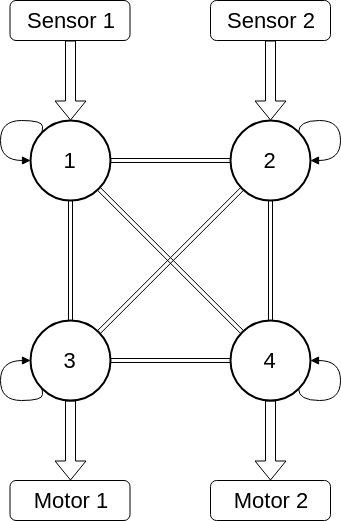
\includegraphics[width=0.4\textwidth,height=7cm]{Imagenes/Agent0Controller}
	\caption{Esquema de la estructura del controlador del ``Agente 0''.}
	\label{fig:a0Controller}
\end{figure}

\subsection{Agente 1: agente colectivo aditivo}
Este agente, al igual que el ``Agente 0'', está diseñado para seguir un comportamiento de fototaxis, pero además cuenta con habilidades sociales para interactuar con el resto de agentes. Las capacidades sociales del agente se han diseñado
e implementado asumiendo que las habilidades cerebrales de los seres vivos pueden interpretarse como módulos independientes que se entrenan por separado. Es decir, que el comportamiento social del agente se encuentra aislado del comportamiento
individual del mismo, y sus evoluciones son por ello independientes.

El agente obtiene lecturas de los mismos sensores usados para la fototaxis, sobre las posiciones del resto de agentes que puede ver, pero estas lecturas son procesadas por una red independiente y por tanto no conectadas a la red de navegación.

\subsubsection{Controlador}
El controlador de este agente es similar al del ``Agente 0'', una red CTRNN de 4 neuronas completamente interconectadas. Aunque al contar con habilidades sociales, se ha añadido una capa independiente de 2 neuronas que será la encargada
de procesar las lecturas de los sensores sobre las posiciones de los agentes y de transmitir la señal adecuada a los motores del agente. Como puede verse en la figura \ref{fig:a1Controller}, las neuronas 1 y 2 están conectadas a los
sensores y se encargan de recibir mediciones de luz y de procesarlas. Las neuronas 5 y 6 están conectadas a los motores, igual que en el Agente 0. Las neuronas 3 y 4 se encargan de procesar las señales de los sensores sobre el posicionamiento
del resto de agentes, procesarlas y transmitir su salida a los motores. Los motores juntan las salidas de las neuronas 3, 4, 5 y 6 para generar una velocidad.

\begin{figure}[H]
	\centering
	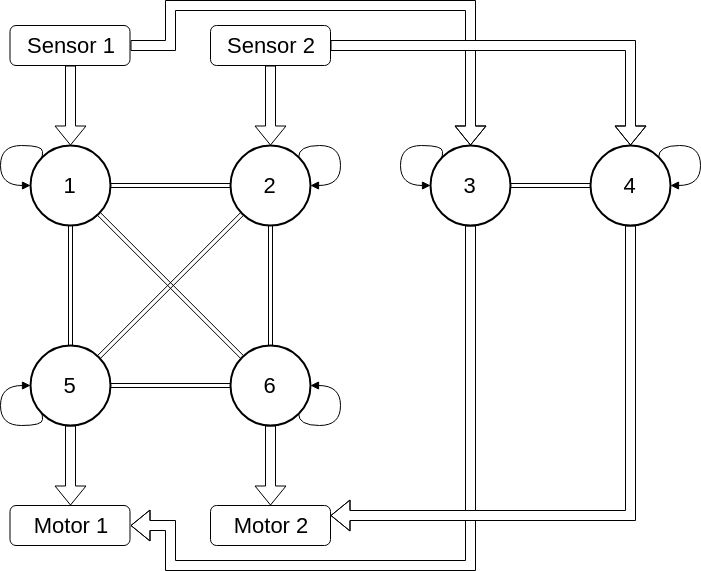
\includegraphics[width=0.6\textwidth,height=7cm]{Imagenes/Agent1Controller}
	\caption{Esquema de la estructura del controlador del ``Agente 1''.}
	\label{fig:a1Controller}
\end{figure}

\subsection{Agente 2: agente colectivo estructural}
El controlador de este agente es una extensión del controlador del ``Agente 0''. A la red CTRNN de 4 neuronas se le han añadido 2 neuronas más, las cuales están conectadas a los sensores y se encargan de procesar las mediciones sobre el posicionamiento
del resto de agentes. La diferencia con el ``Agente 1'' es que estas dos neuronas extra que están interconectadas completamente con el resto de la red, no son independientes. Esta implementación simularía que las capacidades cerebrales de los seres vivos
puedes aprenderse y evolucionar en momentos diversos de su vida, pero esta evolución afecta al resto de neuronas haciéndolas cambiar también. Por tanto, en el ``Agente 2'', el comportamiento social no se encuentra aislado del comportamiento de fototaxis.
\subsubsection{Controlador}
El controlador de este agente es similar al del ``Agente 1'', salvo porque la cada extra de 2 neuronas no se encuentra aislada del resto, sino mezclada con ellas. Como puede verse en la figura \ref{fig:a2Controller}, las neuronas 1 y 2 están conectadas
a los sensores y se encargan de recibir mediciones de luz y de procesarlas. Las neuronas 3 y 4 están conectadas a los sensores y se encargan de procesar las señales de los sensores sobre el posicionamiento del resto de agentes, pero se encuentran completamente
interconectadas con el resto de neuronas. Las neuronas 5 y 6 generan las salidas que los motores convierten en velocidades.

\begin{figure}[H]
	\centering
	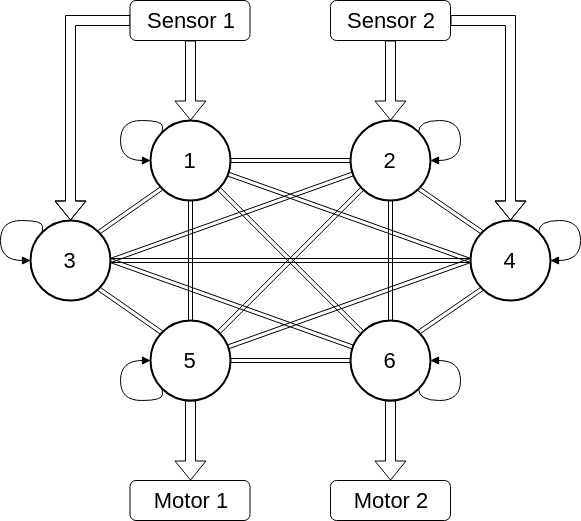
\includegraphics[width=0.5\textwidth,height=7cm]{Imagenes/Agent2Controller}
	\caption{Esquema de la estructura del controlador del ``Agente 1''.}
	\label{fig:a2Controller}
\end{figure}

\section{Evolución}
Para la evolución de los tres tipos de agentes anteriormente descritos se ha implementado un algoritmo genético. El algoritmo es común para los tres agentes, pero algunas de las funciones varían entre los tres tipos para adaptarse a sus estructuras, características y
objetivos propios.

\subsection{Codificación de los agentes}
Cada agente candidato es codificado como un vector que contiene cada uno de sus atributos. El ``Agente 0'' se codifica como un vector de 46 componentes formado por 42 componentes reales y 4 componentes enteras, como puede verse en la figura \ref{fig:vector0}.

\begin{figure}[H]
	\centering
	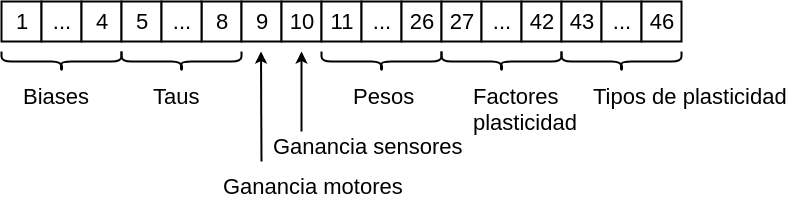
\includegraphics[width=1.0\textwidth,height=4cm]{Imagenes/vector0}
	\caption{Representación codificado de un cromosoma que representa un agente de tipo 0.}
	\label{fig:vector0}
\end{figure}

Los agentes de tipo 1 y 2 estan formados por 6 neuronas, a diferencia de los agentes de tipo 0 que están compuestos por 4 neuronas. Esto hace que el vector de un ``Agente 1'' o de un ``Agente 2'' este formado por 92 elementos, siendo 86 de ellos reales
y 6 enteros, como puede verse en la figura \ref{fig:vector12}

\begin{figure}[H]
	\centering
	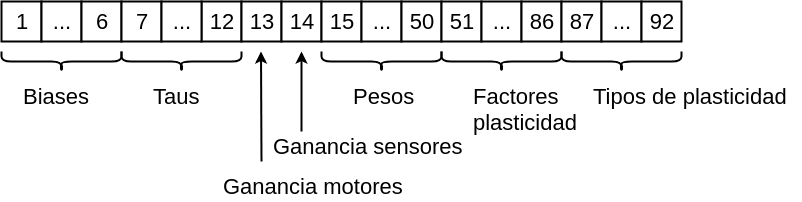
\includegraphics[width=1.0\textwidth,height=4cm]{Imagenes/vector12}
	\caption{Representación codificado de un cromosoma que representa un agente de tipo 1 o 2.}
	\label{fig:vector12}
\end{figure}

Todas las componentes reales de los agentes codificados estan formadas por valores entre [0, 1], los cuales serán escalados a sus rangos establecidos a la hora de evaluar el agente. Las componentes enteras estan formadas por valores del 0 al 3, y
representan los tipos de plasticidad nombrados en el apartado de plasticidad de este documento.

\subsection{Creación de la población inicial}
Para la creación de la población inicial se llama $N$ veces a la función de creación de candidato. Esto da como resultado una población de candidatos aleatorios que constituyen la primera generación.

Se ha seleccionado un tamaño de población inicial ($N$) de \textbf{60} candidatos. Este tamaño se mantiene para el resto de las poblaciones de las siguientes generaciones.

\subsection{Función de selección}
La función de selección es la encargada de elegir los candidatos que serán utilizados para engendrar una nueva generación. Existen muchas formas de seleccionar estos candidatos (de manera aleatoria, los $k$ mejores, los $k$ peores, etc.). En este caso
se ha elegido utilizar la llamada ``selección por torneo''. Este tipo de selección consiste en elegir de manera aleatoria un número determinado de candidatos de entre la población inicial para ``participar en el torneo'', el ganador del torneo es el candidato
con mejor fitness de entre los participantes, el cual es seleccionado para engendrar la nueva generación. El torneo se repite hasta que se han elegido ganadores suficientes como para formar una nueva generación.

Se ha elegido este tipo de selección ya que, por una parte selecciona a aquellos candidatos de la generación actual que mejor fitness han conseguido (quedándote con los mejores), mientras que permite que candidatos menos buenos puedan ser también elegidos como ganadores
(por ejemplo, si los participantes elegidos aleatoriamente son aquellos con peores valores de fitness). El permitir que no solamente los candidatos mejores engendren dota de cierta riqueza al algoritmo genético, permitiendo explorar un mayor abanico de posibilidades
que, quedándonos solo con los mejores, no sería posible explorar.

En nuestro algoritmo genético, el número de participantes en los torneos se ha fijado en \textbf{10} candidatos.

\subsection{Función de recombinación}
La función de recombinación o \textit{crossover} se encarga de crear nuevos individuos a partir de los candidatos seleccionados con la función de selección. En nuestro caso, esta recombinación se aplica con una probabilidad del \textbf{50\%}. En ella se eligen dos candidatos aleatorios de la nueva
generación y se aplica el llamado ``\textit{crossover} uniforme''. En este tipo de recombinación, para cada componente del vector de componentes, los dos candidatos elegidos intercambian sus valores con una cierta probabilidad. El resultado son dos nuevos candidatos formados por componentes de los
elegidos.

En nuestro caso, la probabilidad de que los dos candidatos elegidos intercambien el valor de una componente es del \textbf{0.5}.

\subsection{Función de mutación}
La función de mutación se encarga de aplicar un cierto nivel de aleatoriedad en los candidatos, dando lugar a una mayor riqueza de individuos y una mayor amplitud de resultados posibles. En nuestro caso se ha optado por una mutación básica, la cual se da con una probabilidad del \textbf{50\%}.
La mutación consiste en recorrer el vector de componentes del candidato elegido para mutar, generando un nuevo valor (dentro de sus rangos establecidos) aleatorio para cada componente con una cierta probabilidad.

En nuestro caso, la probabilidad de generar un nuevo valor para una componente real es del \textbf{0.5}, mientras que para una componente entera es del \textbf{0.1}.

\subsection{Función fitness}
La función fitness es la encargada de evaluar a los agentes candidatos, por lo que es de gran importancia tanto que la función represente bien el estado inicial y unos objetivos que alcanzar, como que la forma de puntuar positiva y negativamente a los candidatos según sus resultados sea la adecuada
y refleje correctamente el grado de cumplimiento de los objetivos especificados. Una función fitness adecuada dará como resultado mejores candidatos y puede significar un tiempo de convergencia menor ante una función fitness menos adecuada.

En este proyecto ha sido necesario diseñar e implementar dos funciones fitness. La primera es utilizada por el ``Agente 0'' y se centra en desarrollar comportamientos de fototaxis individual. La segunda es utilizada por el ``Agente 1'' y el ``Agente 2'' y se centra en desarrollar comportamientos de fototaxis
colectiva, es decir, teniendo en cuenta a más de un agente a la vez. Las puntuaciones fitness están acotadas entre 0 y 1.

\subsubsection{Fitness individual}
En un espacio de dos dimensiones, el agente candidato es situado inicialmente en el punto central $(0, 0)$. Durante la ejecución, aparecen \textbf{6} luces hacia las que el agente debe aprender a acercarse. Sólamente habrá una luz encendida a la vez, la cual permanecerá en el espacio durante un número
de iteraciones elegidas aleatoriamente del intervalo $[0.75T, 1.25T]$, teniendo $T=1600$. Cuando una luz se apaga, se genera otra a una distancia $D \in [10R:25R]$ de la posición actual del agente, siendo $R$ el radio del agente. La intensidad ($I$) que emite la luz se elige en el momento de su creación aleatoriamente de manera que
$I = [500, 1500]$.

Para el entrenamiento individual se busca recompensar tres comportamientos, los cuales se utilizarán para calcular la puntuación fitness de cada agente al finalizar la ejecución:
\begin{enumerate}
	\item{Que para cada luz, el agente acabe más cerca de ella de lo que empezó.}
	\item{Que para cada luz, el agente permanezca el mayor número de iteraciones posibles a menos de una distancia a partir de la que se considera que el agente está cerca ($D_{\text{ok}} = R*4$, siendo $R$ el radio del agente).}
	\item{Que para cada luz, el agente mantenga el mayor número de sus neuronas estables.}
\end{enumerate}

Por tanto, nuestra puntuación fitness estará formada por tres factores; $Fd$ para el comportamiento de acercamiento, $Fp$ para el comportamiento de permanencia cerca de la luz y $Fh$ para el comportamiento de estabilidad. Para cada luz, en el instante que se apague se calculará la puntuación
que el agente ha obtenido en ella mediante las fórmulas \ref{eq:FdIndi} (siendo $D_{f}$ la distancia final y $D_{i}$ la distancia inicial entre el agente y la luz), \ref{eq:FpIndi} y \ref{eq:FhIndi}.

\begin{equation} \label{eq:FdIndi}
	Fd=\begin{cases}
0.0 & \text{ IF }\quad D_{f} > D_{i}  \\
1 - (D_{f} / D_{i}) & \text{ IF }\quad D_{f} \leq D_{i} \\
\end{cases}
\end{equation}


\begin{equation} \label{eq:FpIndi}
 \centering
	Fp = \frac{\text{Nº ciclos cerca de la luz}}{\text{Nº de ciclos que la luz ha estado encendida}}
\end{equation}

\begin{equation} \label{eq:FhIndi}
 \centering
	Fh = \frac{\text{Nº neuronas que no han perdido estabilidad}}{\text{Nº de neuronas del agente}}
\end{equation}

La puntuación final del agente para esa luz será una suma ponderada de los factores, de forma que se da más peso a aquellos que se consideran más importantes, como puede verse en la ecuación \ref{eq:fitnessIndi}.
\begin{equation} \label{eq:fitnessIndi}
 \centering
	fitness = (0.34Fd + 0.54Fp + 0.12Fh)
\end{equation}

Una vez obtenida la puntuación fitness del agente para cada una de las 6 luces, la fitness total se corresponde con su media, siendo esa la puntuación final del agente.

\subsubsection{Fitness colectiva}
En la fitness colectiva, el funcionamiento del sistema de luces y los parámetros del mismo son iguales a los de la fitness individual. Sin embargo, algunos aspectos cambian. Al ser un experimento colectivo ya no tenemos un único agente, sino \textbf{5}. Al comienzo se situan a una determinada distancia
del centro del espacio, que se selecciona de forma aleatoria del intervalo $[4R, 8R]$ siendo $R$ el radio del agente, y con una orientación también aleatoria. A diferencia de la fitness individual, en la fitness colectiva las luces se generan a una distancia $D \in [10R, 25R]$ del centroide
formado por los agentes, siendo $R$ el radio del agente. Además, los agentes con comportamientos colectivos perciben al resto de agentes de forma similar a como perciben las luces (cada agente tiene una intensidad que en función de la distancia a la que se encuentre del sensor que lo lee producirá una señal
más fuerte o más suave). La intensidad ($I_{agente})$ que emite cada agente es un valor fijo $I_{agente} = 750$.

En el entrenamiento colectivo se busca recompensar tres comprtamientos, los cuales se utilizarán para calcular la puntuación fitness del grupo de agentes:
\begin{enumerate}
	\item{Que para cada luz, cada agente acabe más cerca de ella de lo que empezó.}
	\item{Que para cada luz, se respete correctamente la restricción colectiva añadida.}
	\item{Que para cada luz, cada agente mantenga el mayor número de sus neuronas estables.}
\end{enumerate}

Como podemos observar, el segundo comportamiento buscado es distinto al del entrenamiento individual. Este nuevo factor premiará que los agentes se mantengan cerca de la luz que se encuentre actualmente encendida el mayor número de ciclos posible, pero con una restricción colectiva añadida que consiste
en que sólamente \textbf{3} agentes pueden estar cerca de una luz simultáneamente. Se utilizará un contador colectivo para llevar el control de este comportamiento, de manera que cuando un agente se encuentre cerca de la luz y el total de agentes cerca de esa luz sea menor que 3, aumentará el contador en una unidad. Sin
embargo, si el número de agentes que se encuentran a la vez cerca de la luz excede del límite de 3, se considera que todo el conjunto de agentes ha fallado y se disminuirá el contador en 5 unidades (una unidad por cada agente del grupo). El máximo de puntuación que el conjunto de agentes puede obtener en el comportamiento colectivo para una
luz es de ($3 * \text{Ciclos luz encendida}$), que sería el resultado de que durante todo el tiempo que la luz ha estado encendida, sólo 3 agentes hayan estado cerca.

Por tanto, nuestra puntuación fitness estará formada por tres factores; $Fd$ para el comportamiento de acercamiento, $Fp$ para el comportamiento colectivo y $Fh$ para el comportamiento de estabilidad. Al finalizar la última luz se calculará la puntuación
que el conjunto de agentes ha obtenido mediante las fórmulas \ref{eq:FdColectiva} (siendo $D_{fk}$ la distancia final del agente $k$ y $D_{ik}$ la distancia inicial del agente $k$, entre el él y la luz), \ref{eq:FpColectiva} y \ref{eq:FhColectiva}.

\begin{equation} \label{eq:FdColectiva}
	Fd = \frac{\sum_{k=1}^{5}(\frac{\sum_{j=1}^{NºLuces}Fd_{kj}}{NºLuces})}{5} \qquad \Rightarrow \qquad Fd_{kj}=\begin{cases}
	0.0 & \text{ IF }\quad D_{fkj} > D_{ikj}  \\
	1 - (D_{fkj} / D_{ikj}) & \text{ IF }\quad D_{fkj} \leq D_{ikj} \\
	\end{cases}
\end{equation}

\begin{equation} \label{eq:FpColectiva}
 \centering
		Fp = \frac{\sum_{i= 1}^{\text{NºLuces}}\text{Contador}_{i}}{(\sum_{i =1}^{\text{NºLuces}}\text{Ciclos encendida}_{i}) * 3}
\end{equation}

\begin{equation} \label{eq:FhColectiva}
 \centering
		Fh = \frac{\sum_{i = 1}^{Nº Luces}\frac{\sum_{k=1}^{5}(\frac{\text{Nº neuronas que no han perdido estabilidad}_{ki}}{\text{Nº de neuronas del agente}_{ki}})}{5}}{Nº Luces}
\end{equation}

Una vez obtenidos estos valores, se ponderan y se obtiene la fitness total del conjunto de agentes (\ref{eq:fitnessCol}).
\begin{equation} \label{eq:fitnessCol}
 \centering
	fitness = (0.44Fd + 0.44Fp + 0.12Fh)
\end{equation}

\section{Simetría}
Las redes CTRNN que actúan como controladores de los agentes cuentan con simetría en las ganancias de los motores y los sensores. Esto quiere decir que ambos motores comparten el mismo valor para la ganancia y que ambos sensores
comparten el mismo valor para la ganancia.

\section{Parámetros y rangos}
Para todos los agentes anteriormente descritos, los rangos establecidos para sus variables internas pueden verse en la tabla \ref{table:tablaValoresParametros}.
\begin{table}[H]
\centering
\begin{tabular}{l|l|c|c}
\textbf{Parametro} & \textbf{Descripción}          & \multicolumn{1}{l|}{\textbf{Valor mínimo}} & \multicolumn{1}{l}{\textbf{Valor máximo}} \\
\textit{$\tau_{i}$}       & Constante de decaimiento      & 0.4                                        & 4.0                                       \\
\textit{$\theta{i}$}      & Bias                          & -3.0                                       & 3.0                                       \\
\textit{Gain}      & Ganancia motora y sensora     & 0.1                                        & 10.0                                      \\
\textit{$w_{ij}$}      & Peso de la conexión sináptica & -10.0                                      & 10.0                                      \\
\textit{$n_{ij}$}     & Ritmo de plasticidad          & -0.9                                       & 0.9
\end{tabular}
\caption{Rango de valores para los parámetros de la red}
 \label{table:tablaValoresParametros}
\end{table}

\chapter{Experimentos}

\chapter{Conclusiones}

\chapter{Conclusiones personales}

Este proyecto me ha permitido introducirme más en un área en la que estoy enormemente interesado y de la que, desgraciadamente, no he aprendido tanto como me gustaría durante la carrera, la Inteligencia Artificial. En un futuro
me gustaría seguir por este camino y aprender más sobre esa temática.

Aprovecho para agradecer a Manuel Gonzalez Bedía, director de este proyecto, su involucración e interés desde el día de comienzo. He podido contar con él en cualquier momento que lo haya podido necesitar y su pasión y conocimientos me han introducido
en un mundo científico del que me gustaría seguir aprendiendo.


%Puedes añadir más capítulos
%%%%%%%%%%%%%%%%%%%%%%%%%%%%%%%%%%%%%%%%%%%%%%%%%%%%%%%%%%%%%%%%%%%%%%%%%%%%%%%%%%%
%		BIBLIOGRAFÍA Y REFERENCIAS
%%%%%%%%%%%%%%%%%%%%%%%%%%%%%%%%%%%%%%%%%%%%%%%%%%%%%%%%%%%%%%%%%%%%%%%%%%%%%%%%%%%

\bibliographystyle{unsrt} %plaindin
\bibliography{Capitulos/Bibliografia}
\nocite{*}



%%%%%%%%%%%%%%%%%%%%%%%%%%%%%%%%%%%%%%%%%%%%%%%%%%%%%%%%%%%%%%%%%%%%%%%%%%%%%%%%%%%
%		ANEXOS
%%%%%%%%%%%%%%%%%%%%%%%%%%%%%%%%%%%%%%%%%%%%%%%%%%%%%%%%%%%%%%%%%%%%%%%%%%%%%%%%%%%

\newpage
\appendix
\clearpage
\addappheadtotoc
\appendixpage
\chapter{Homeostat}\label{ch:anexo1}
Para comprender mejor los fundamentos de la homeostasis se diseñó e implementó un Homeostat en el lenguaje de programación Python siguiendo los fundamentos teóricos descritos en el punto explicativo de la homeostasis en este
mismo documento.

Para ello, se implementó una sencilla red de 4 neuronas totalmente interconectadas. En cada iteración, cada neurona recibe una serie de entradas del resto de neuronas y de ella misma. El peso de estas entradas está definido
por la fuerza de conexión entre ellas. El sumatorio ponderado de estas entradas sobre una neurona determina su salida $s_{i}$.

Al comienzo, los pesos de la fuerza de las conexiones están distribuidos de forma aleatoria dentro de los rangos apropiados $R = [0.5 - \alpha, \alpha + 0.5]$, donde $\alpha$ determina la opresión de la restricción homeostática.
Tras cada iteración, si $s_{i} \in R$, la neurona es estable. Si $s_{i} \notin R$ la neurona ha perdido la estabilidad y se activa el mecanismo de cambio adaptativo.

En cuanto se detecta que una neurona ha salido del rango de estabilidad sus parametros comienzan a variar de forma aleatoria (pero dentro de los limites establecidos para cada parametro) hasta que la neurona vuelve a la estabilidad.

La finalidad de este experimento es la comprobar como al comienzo, las neuronas del sistema se podían encontrarse fuera de los rangos de estabilidad (debido a que al principio sus parametros tienen valores aleatorios), pero tras una
serie de iteraciones todas las neuronas se estabilizan.

En la figura \ref{fig:customHomeostat} podemos ver una gráfica que refleja el funcionamiento del Homeostato. En ella, cada linea de color representa la salida de una de las neuronas que componen el Homeostato. Como podemos observar,
al comienzo, partiendo de valores aleatorios en los parámetros, las salidas son inestables y se encuentran fuera del rango establecido. Podemos observar como la neurona representada con el color verde es la última que se estabiliza. Es interesante
también observar como las neuronas se influyen entre ellas durante este proceso de estabilización. Esto puede verse en el último pico ascendente de la neurona representada con el color verde, el cual provoca un ligero movimiento en la
salida de la neurona representada con el color azul, la cual no llega a desestabilizarse (la neurona verde arrastra a la azul con algunos de sus movimientos). Al cabo de un tiempo, todas las neuronas consiguen estabilizarse dentro
del rango establecido. Una vez estables, sin la existencia de ninguna perturbación que provoque la salida de alguna de ellas de la zona de estabilidad, se mantendrán inmutables indefinidamente.

\begin{figure}[H]
    \centering
    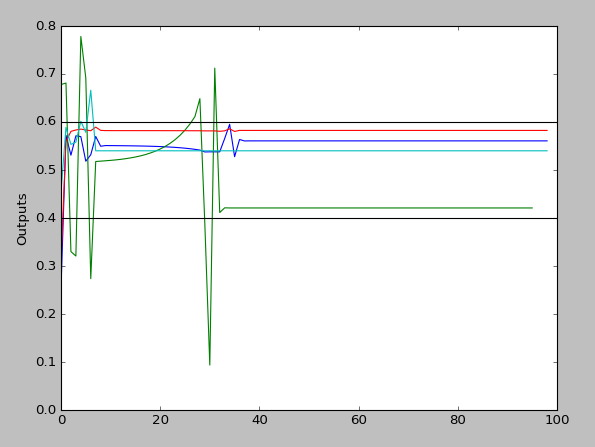
\includegraphics[width=0.8\textwidth,height=8cm]{Imagenes/CustomHomeostat}
    \caption{Gráfica de salidas del Homeostato implementado. \textbf{Eje X:} tiempo. \textbf{Eje Y: } salidas de cada una de las neuronas que componen el Homeostato.}
    \label{fig:customHomeostat}
\end{figure}

\chapter{Algoritmo genético}\label{ch:anexo2}
Los algoritmos genéticos son un tipo de algoritmos de optimización, lo que quiere decir que se utilizan para
obtener la solución o soluciones óptimas de un problema computacional\cite{JennaCarr}.

Estos algoritmos representan una rama dentro del campo conocido como ``Computación evolutiva''. En ella, se
imitan los procesos biológicos de reproducción y selección natural con el fin de encontrar la mejor solución al
problema para el que son creados. Al igual que en la evolución, muchos de los procesos de un algoritmo genético son
aleatorios, aunque las técnicas de optimización permiten limitar el nivel de aleatoriedad y adaptar el control sobre
el algoritmo que se considere necesario.

Este tipo de algoritmos permiten encontrar soluciones a problemas que otros algoritmos de optimización no pueden calcular
por falta de continuidad, derivabilidad, linealidad u otras características.

\subsection{Componentes, estructura y terminología}
Dado que los algoritmos genéticos están diseñados para simular procesos biológicos, gran parte de su terminología ha sido tomado
prestada de la biología. A pesar de ello, las entidades a las que esta terminología se refieren en el entorno de los algoritmos genéticos
son mucho más simples que sus equivalentes biológicos. Los componentes básicos de prácticamente todos los algoritmos genéticos son:

\begin{itemize}
	\item{Una función \textbf{fitness} para la optimización}
	\item{Una \textbf{población} de \textbf{cromosomas}}
	\item{Una función de \textbf{selección} para elegir los cromosomas que van a reproducirse}
	\item{Una función de \textbf{recombinación} (o \textit{crossover}) para la producción de la siguiente generación de cromosomas}
	\item{Una función de \textbf{mutación} para aleatorizar algunos cromosomas de la nueva población}
\end{itemize}

La \textit{función fitness} es la función que el algoritmo está tratando de optimizar. La palabra ``fitness'' se toma prestada de la teoría evolutiva.
Se utiliza porque la función de fitness testea y valora como de buena (como de ``\textit{fit}'') es cada solución potencial del problema. El término
\textit{cromosoma} hace referencia al valor o valores numéricos que representan posibles soluciones candidatas al problema que se está intentando resolver.
Cada cromosoma está formado por una lista de parámetros, llamados \textit{genes}. Al conjunto de cromosomas que van a evaluarse como posibles candidatos a solución
del problema se le llama \textit{población}. Antiguamente los cromosomas eran codificados como listas de unos y ceros (codificación binaria), sin embargo, actualmente la computación
moderna permite codificar los cromosomas como números reales u otros objetos.

\begin{figure}[H]
    \centering
    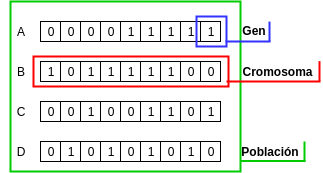
\includegraphics[width=0.6\textwidth,height=5cm]{Imagenes/PoblacionGA}
    \caption{Ejemplo de estructura de población, cromosomas y genes.}
    \label{fig:figuraPoblacionGA}
\end{figure}

Un algoritmo genético comienza con una \textit{población inicial} de cromosomas, generados de forma aleatoria, que representan la primera generación de posibles soluciones. A continuación,
se evalúa cada cromosoma de dicha población mediante la función fitness para comprobar cómo de bien resuelve el problema planteado. Al finalizar, cada candidato tiene asignada una puntuación
de fitness que representa lo bien (o lo mal) que lo ha hecho intentando resolver el problema.
Una vez con la población inicial completamente evaluada, el \textit{operador de selección} escoge de entre toda la población de candidatos algunos cromosomas para la reproducción (creación
de una nueva generación). Existen muchos tipos de algoritmos de selección, pero generalmente en todos ellos se eligen los cromosomas que mejor puntuación fitness han obtenido, buscando que
las siguientes generaciones creadas a partir de ellos den resultados como mínimo igual de buenos a los suyos.
En el siguiente paso, el \textit{operador de recombinación} simula las operaciones de recombinación de cromosomas presentes en las operaciones de división celular de tipo \textit{meiosis}. En la figura
\ref{fig:figuraCrossover} se puede observar un ejemplo de operación de recombinación. En este proceso se seleccionan dos cromosomas de la población y se recombinan para crear dos descendientes.

\begin{figure}[H]
    \centering
    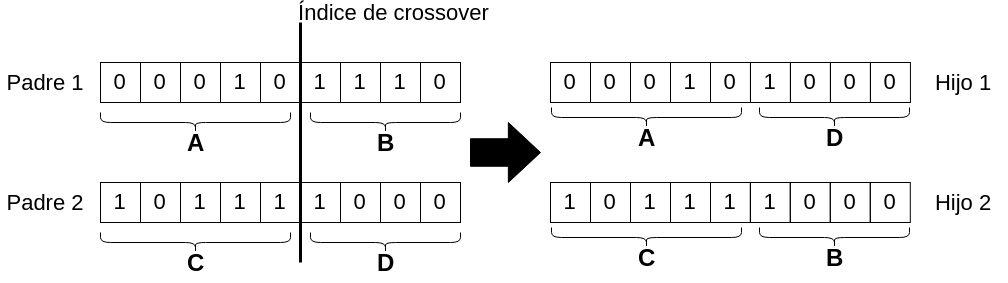
\includegraphics[width=1.0\textwidth,height=5cm]{Imagenes/CrossoverExample}
    \caption{Ejemplo de operación de recombinación de dos cromosomas.}
    \label{fig:figuraCrossover}
\end{figure}

El \textit{operador de mutación} modifica de forma aleatoria genes de los cromosomas descendientes (por ejemplo cambiando un 1 por un 0 y viceversa, en cromosomas binarios). Estas mutaciones ocurren
generalmente con una probabilidad bastante baja. A primera vista, el proceso de mutación puede parecer innecesario e incluso entorpecedor. La realidad es que toma un papel muy importante. Las operaciones
de selección y recombinación mantienen la información genética de los cromosomas con mejor puntuación fitness, pero estos cromosomos sólo son considerados los mejores respecto a la población de la generación
en la que fueron elegidos. Esto puede provocar que el algoritmo converga demasiado rápido y de una solución final alejada de la solución máxima. En otras palabras, puede provocar que el algoritmo se quede
atascado en un máximo local antes de encontrar el máximo global óptimo. El operador de mutación ayuda a proteger el algoritmo de este problema manteniendo la diversidad en la población, a costa de aumentar
el tiempo de convergencia.

Lo normal es que la selección, recombinación y mutación continuen hasta que el numero de descendientes es igual al número de cromosomas de la población inicial, para que esta segunda generación esté compuesta
en su totalidad por descendentienes y reemplace a la población anterior.

Ahora la segunda generación se evalúa mediante la función fitness y todo el proceso se repite. Es una práctica comúm el almacenar el cromosoma con la mayor puntuación de fitness junto con dicha puntuación para
guardar un registro del mejor cromosoma hasta el momento.

Los algoritmos genéticos iteran hasta que la puntuación fitness del mejor cromosoma hasta el momento se estabiliza y no cambia en una serie de generaciones. Esto significa que el algoritmo ha convergido en una
o solución. A todo el proceso de iteraciones se llama \textit{carrera} (en inglés, \textit{run}). Al final de cada carrera se tiene, normalmente, al menos un cromosoma que es una solución lo suficientemente
buena (lo suficientemente \textit{fit}) del problema. Dependiendo del tipo de algoritmo utilizado, la mejor solución puede ser el mejor cromosoma que ha aparecido en todas las iteraciones o el mejor cromosoma
de la última generación.

El rendimiento de un algoritmo genético depende enormemente de los métodos utilizados para codificar posibles soluciones en cromosomas y el criterio utilizado en la función fitness para evaluar a los candidatos.
Otros detalles importantes a tener en cuenta son las probabilidades de recombinación y mutación, el tamaño de la población y el número de iteraciones. Estos valores puedes ser ajustados convenientemente después
de analizar el rendimiento del algoritmo tras unas carreras de prueba.

Los algoritmos genéticos tienen una gran variedad de aplicaciones. Algunos ejemplos destacados son la \textit{programación automática} y el \textit{``machine learning''}. Funcionan también especialmente bien para
modelar distintos fenómenos en economía, ecología, el sistema inmunológico humano, genética y sistemas sociales.

\chapter{Gráficas completas de las activaciones neuronales del grupo de agentes de tipo 1}\label{ch:anexo3}
\begin{figure}[!h]
    \centering % <-- added
\begin{subfigure}{0.33\textwidth}
  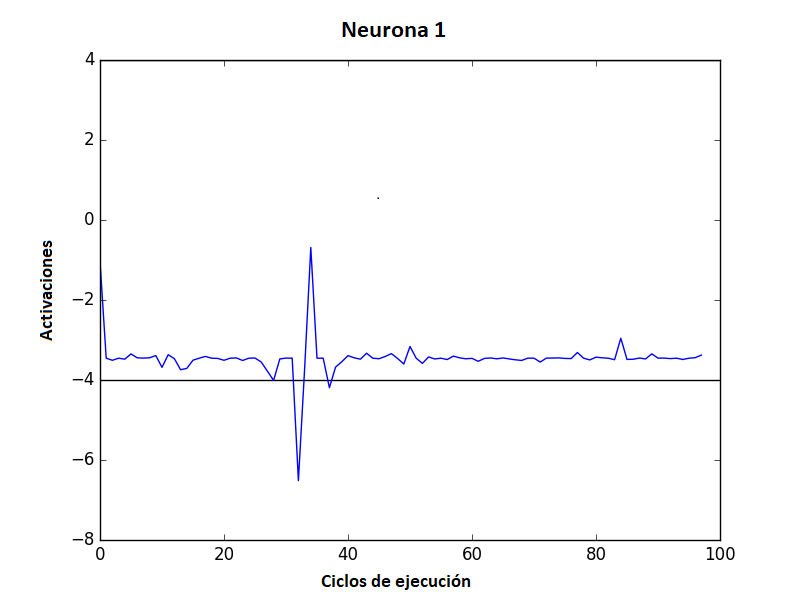
\includegraphics[width=\linewidth]{Imagenes/Agente1Activaciones/Agente0/Neurona0}
\end{subfigure}\hfil % <-- added
\begin{subfigure}{0.33\textwidth}
  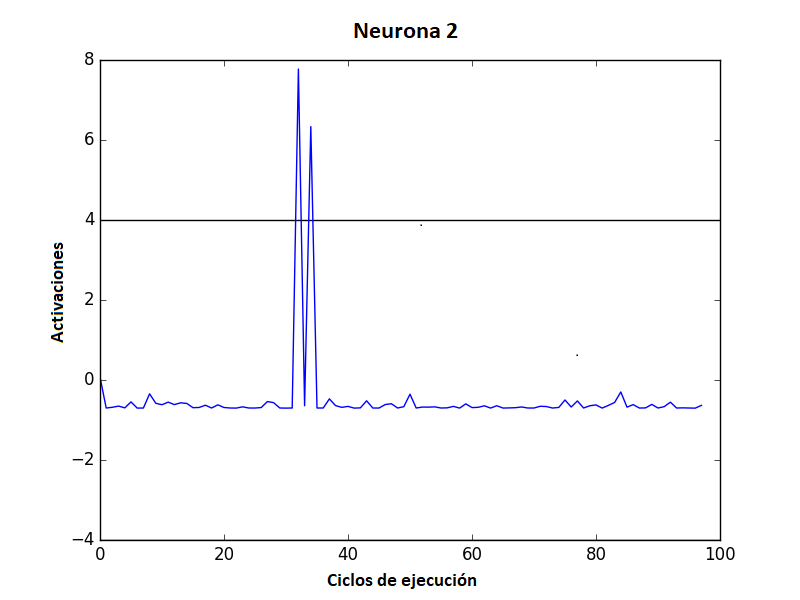
\includegraphics[width=\linewidth]{Imagenes/Agente1Activaciones/Agente0/Neurona1}
\end{subfigure}\hfil % <-- added
\begin{subfigure}{0.33\textwidth}
  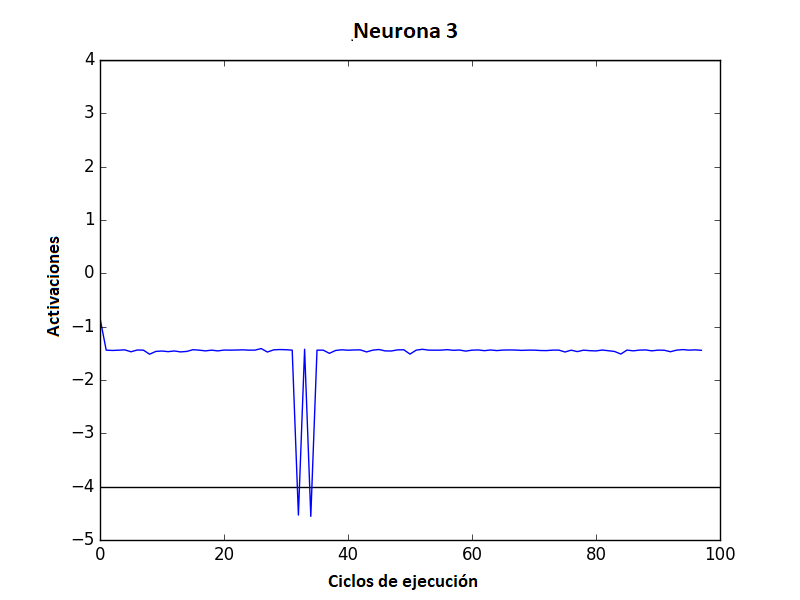
\includegraphics[width=\linewidth]{Imagenes/Agente1Activaciones/Agente0/Neurona2}
\end{subfigure}
\medskip
\begin{subfigure}{0.33\textwidth}
  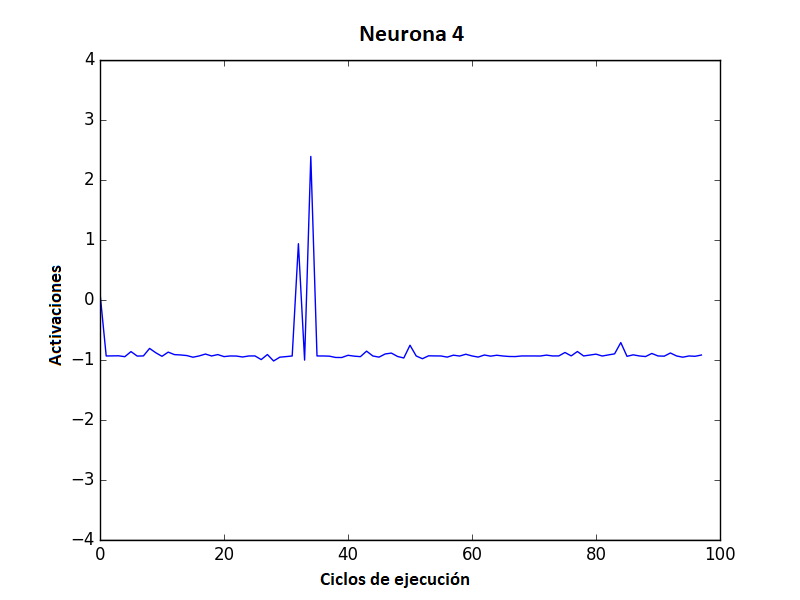
\includegraphics[width=\linewidth]{Imagenes/Agente1Activaciones/Agente0/Neurona3}
\end{subfigure}\hfil % <-- added
\begin{subfigure}{0.33\textwidth}
  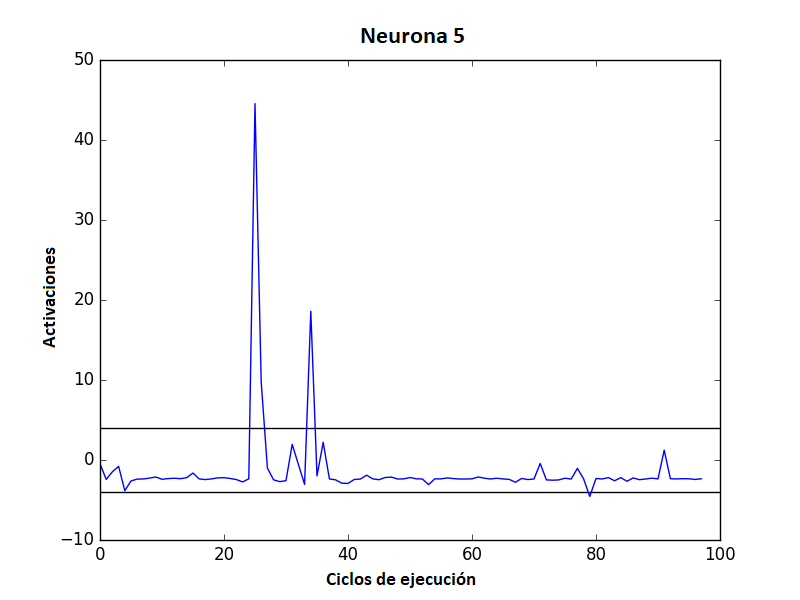
\includegraphics[width=\linewidth]{Imagenes/Agente1Activaciones/Agente0/Neurona4}
\end{subfigure}\hfil % <-- added
\begin{subfigure}{0.33\textwidth}
  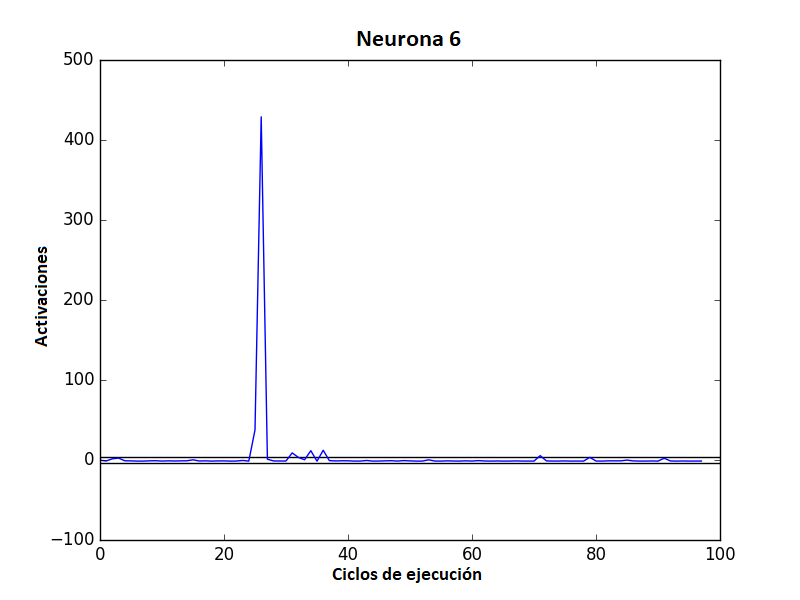
\includegraphics[width=\linewidth]{Imagenes/Agente1Activaciones/Agente0/Neurona5}
\end{subfigure}
\caption{Activaciones de las 6 neuronas del agente número 1 del tipo 1.}
\end{figure}

\begin{figure}[!h]
    \centering % <-- added
\begin{subfigure}{0.33\textwidth}
  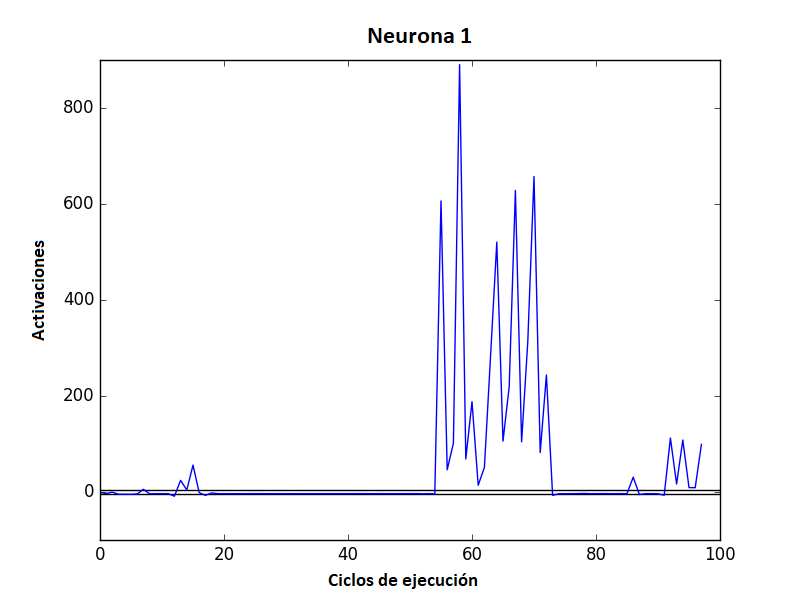
\includegraphics[width=\linewidth]{Imagenes/Agente1Activaciones/Agente1/Neurona0}
\end{subfigure}\hfil % <-- added
\begin{subfigure}{0.33\textwidth}
  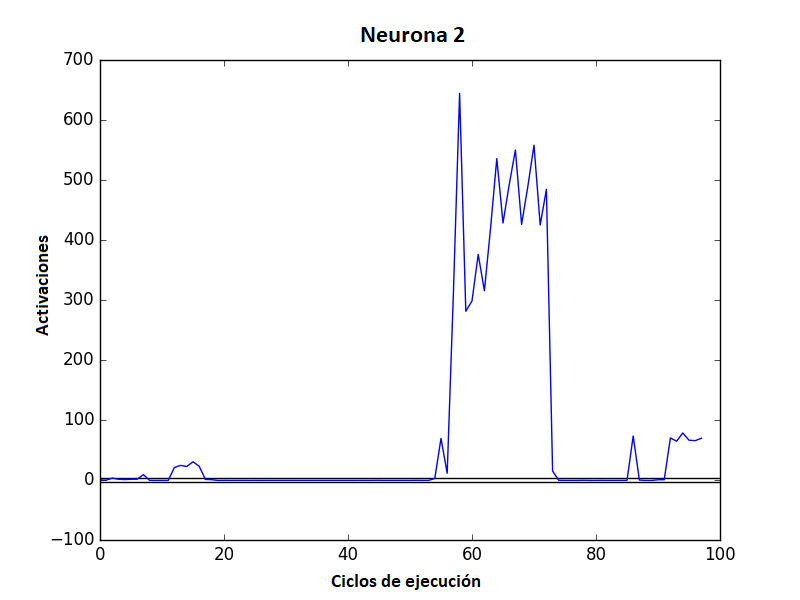
\includegraphics[width=\linewidth]{Imagenes/Agente1Activaciones/Agente1/Neurona1}
\end{subfigure}\hfil % <-- added
\begin{subfigure}{0.33\textwidth}
  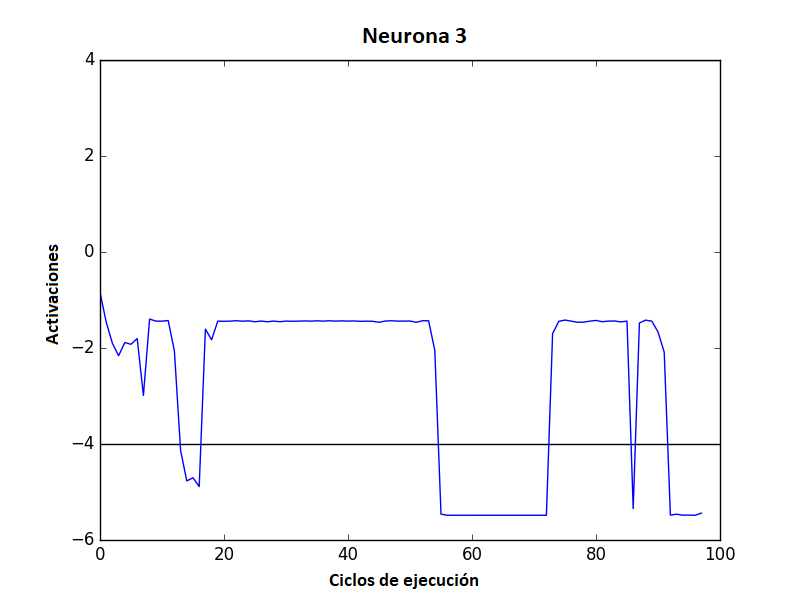
\includegraphics[width=\linewidth]{Imagenes/Agente1Activaciones/Agente1/Neurona2}
\end{subfigure}
\medskip
\begin{subfigure}{0.33\textwidth}
  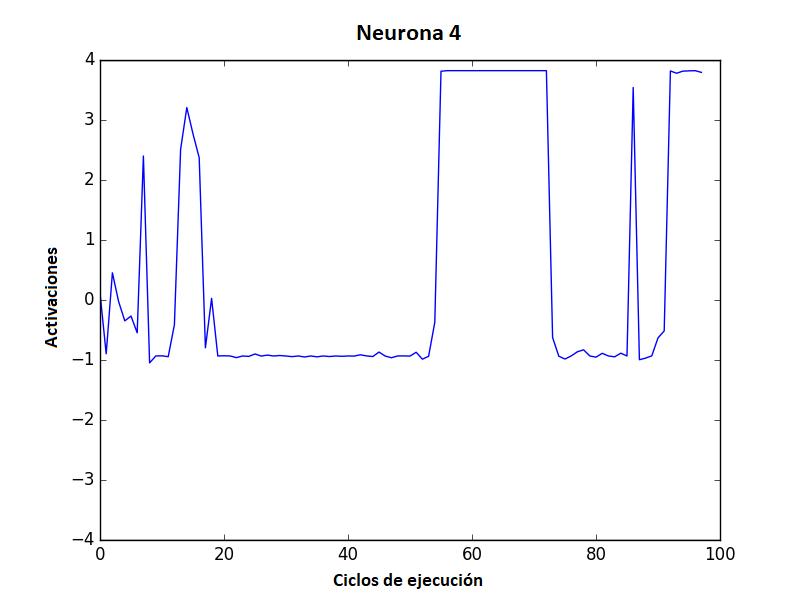
\includegraphics[width=\linewidth]{Imagenes/Agente1Activaciones/Agente1/Neurona3}
\end{subfigure}\hfil % <-- added
\begin{subfigure}{0.33\textwidth}
  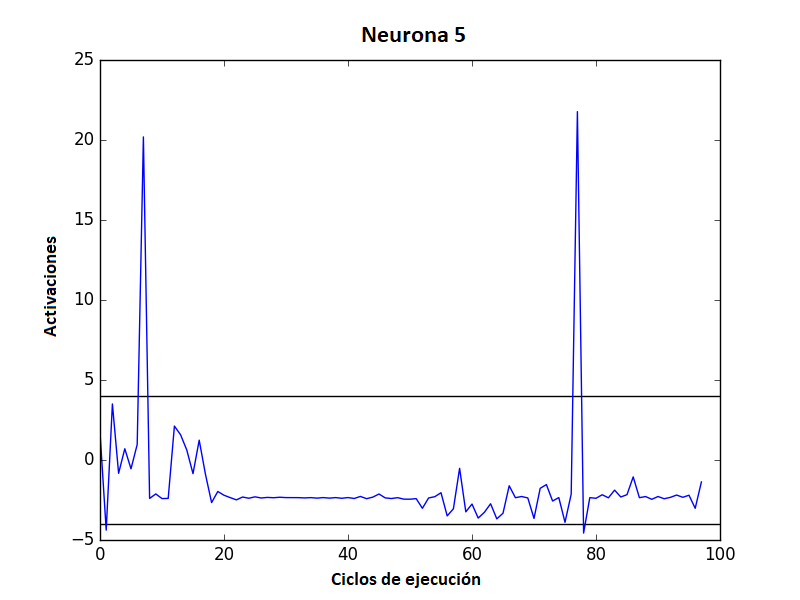
\includegraphics[width=\linewidth]{Imagenes/Agente1Activaciones/Agente1/Neurona4}
\end{subfigure}\hfil % <-- added
\begin{subfigure}{0.33\textwidth}
  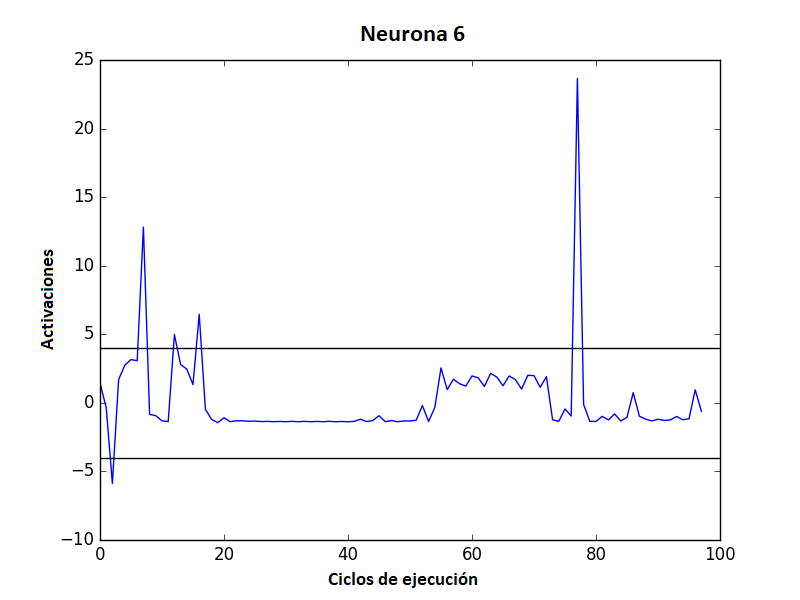
\includegraphics[width=\linewidth]{Imagenes/Agente1Activaciones/Agente1/Neurona5}
\end{subfigure}
\caption{Activaciones de las 6 neuronas del agente número 2 del tipo 1.}
\end{figure}

\begin{figure}[!h]
    \centering % <-- added
\begin{subfigure}{0.33\textwidth}
  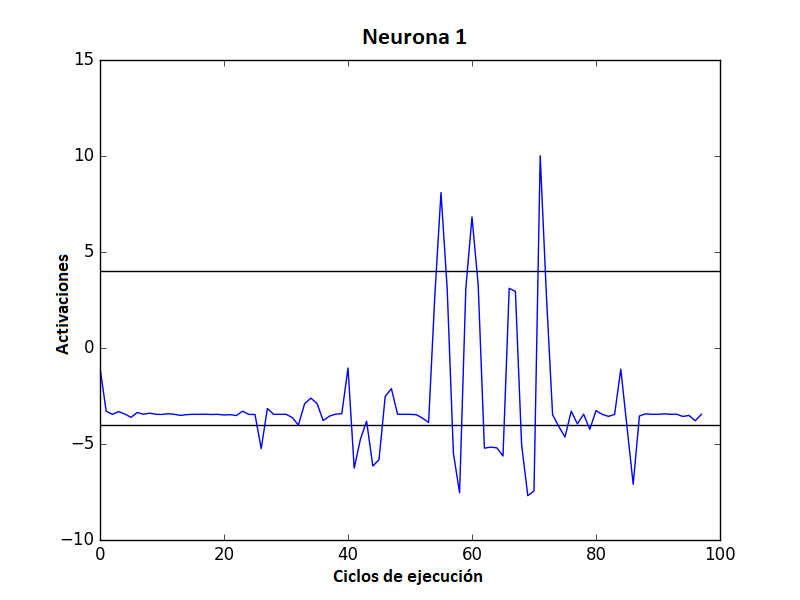
\includegraphics[width=\linewidth]{Imagenes/Agente1Activaciones/Agente2/Neurona0}
\end{subfigure}\hfil % <-- added
\begin{subfigure}{0.33\textwidth}
  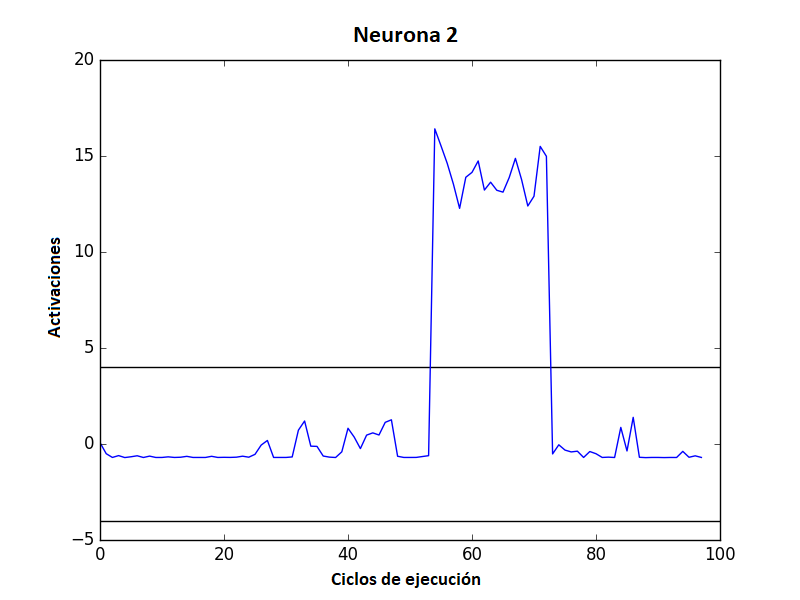
\includegraphics[width=\linewidth]{Imagenes/Agente1Activaciones/Agente2/Neurona1}
\end{subfigure}\hfil % <-- added
\begin{subfigure}{0.33\textwidth}
  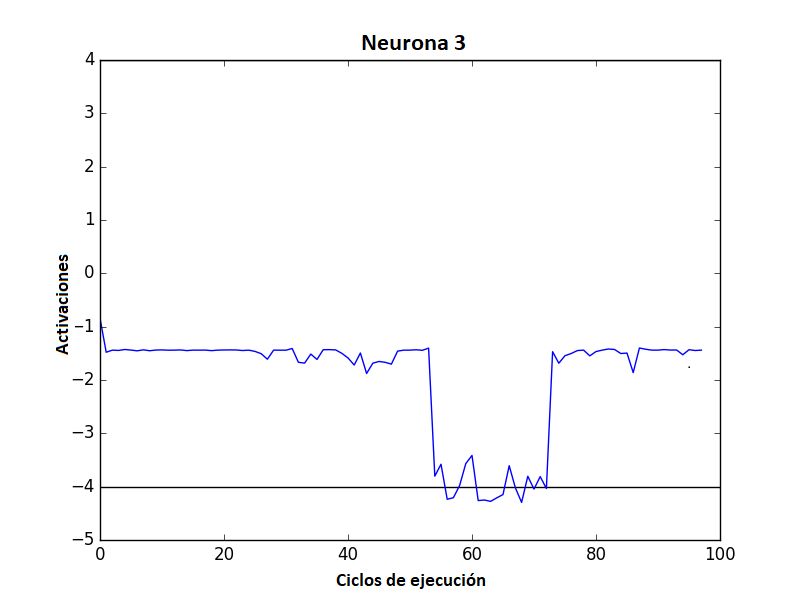
\includegraphics[width=\linewidth]{Imagenes/Agente1Activaciones/Agente2/Neurona2}
\end{subfigure}
\medskip
\begin{subfigure}{0.33\textwidth}
  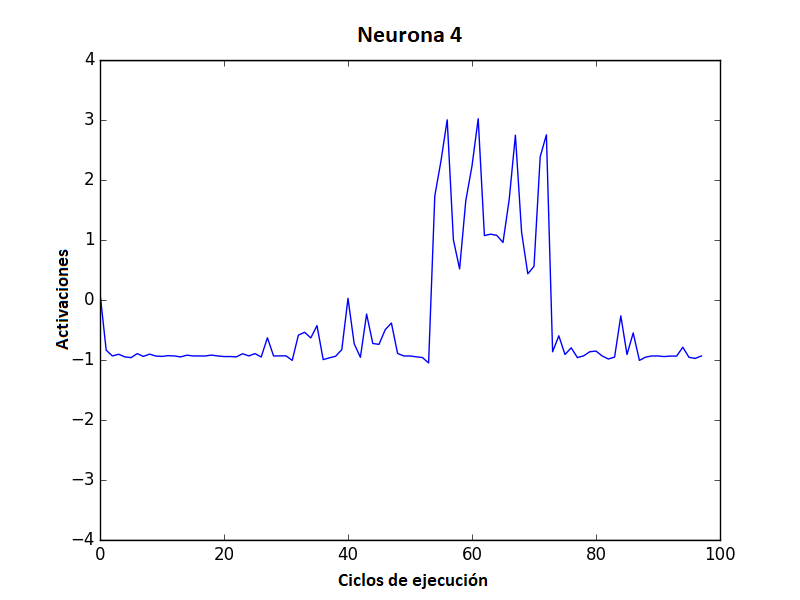
\includegraphics[width=\linewidth]{Imagenes/Agente1Activaciones/Agente2/Neurona3}
\end{subfigure}\hfil % <-- added
\begin{subfigure}{0.33\textwidth}
  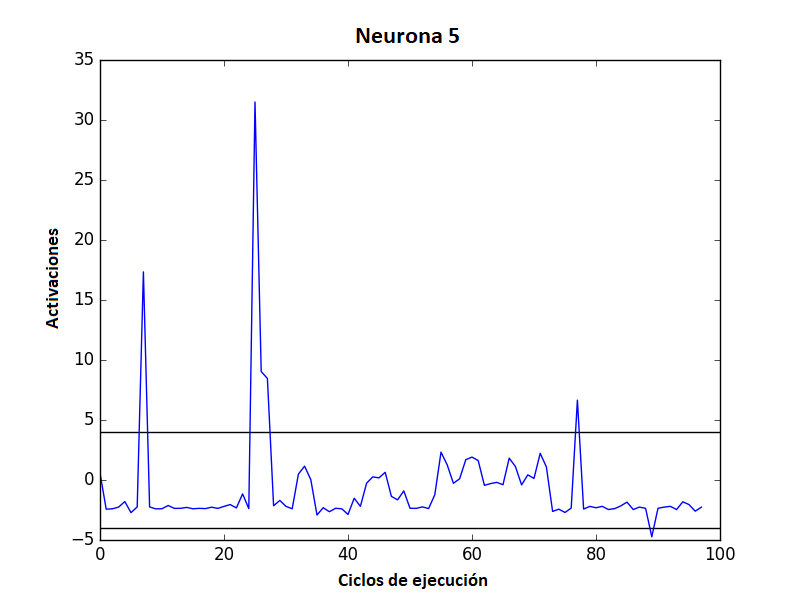
\includegraphics[width=\linewidth]{Imagenes/Agente1Activaciones/Agente2/Neurona4}
\end{subfigure}\hfil % <-- added
\begin{subfigure}{0.33\textwidth}
  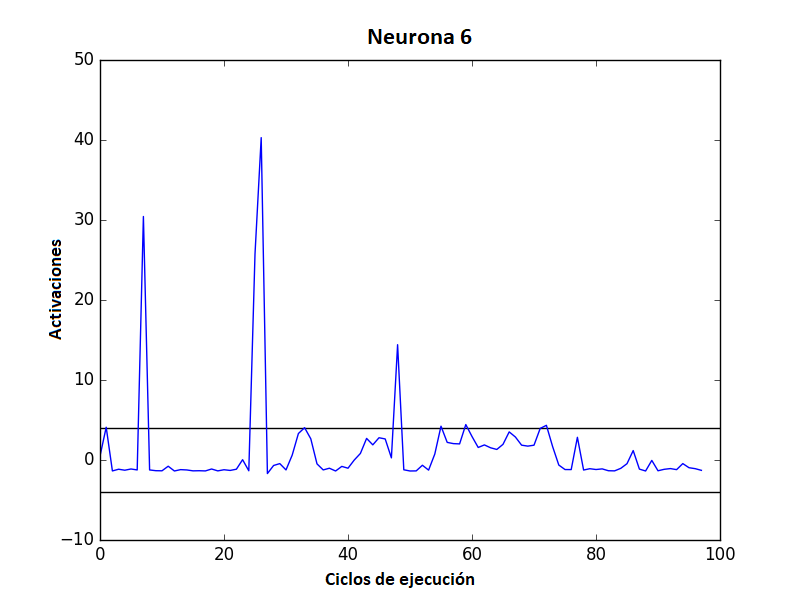
\includegraphics[width=\linewidth]{Imagenes/Agente1Activaciones/Agente2/Neurona5}
\end{subfigure}
\caption{Activaciones de las 6 neuronas del agente número 3 del tipo 1.}
\end{figure}

\begin{figure}[!h]
    \centering % <-- added
\begin{subfigure}{0.33\textwidth}
  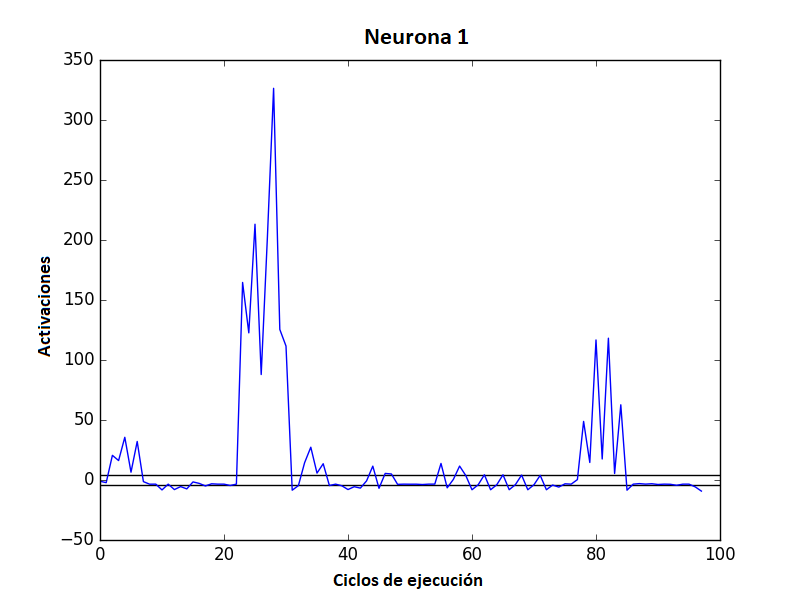
\includegraphics[width=\linewidth]{Imagenes/Agente1Activaciones/Agente3/Neurona0}
\end{subfigure}\hfil % <-- added
\begin{subfigure}{0.33\textwidth}
  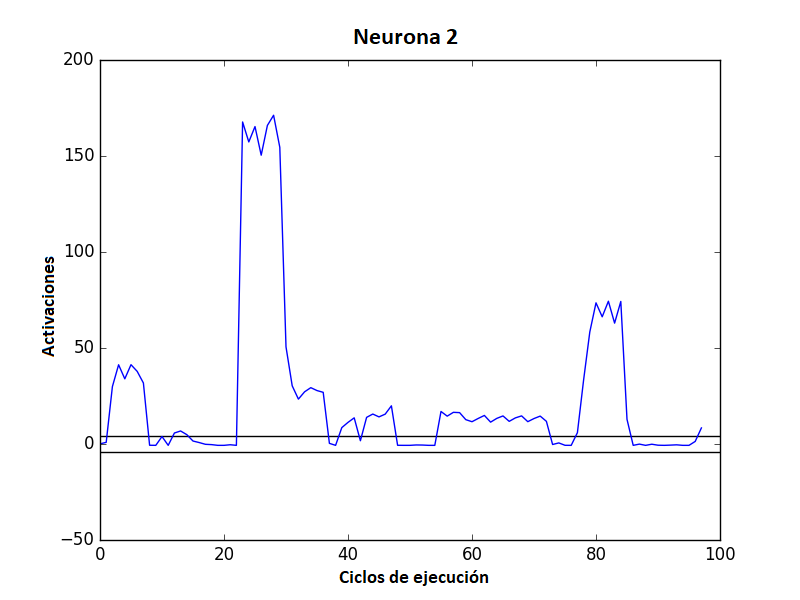
\includegraphics[width=\linewidth]{Imagenes/Agente1Activaciones/Agente3/Neurona1}
\end{subfigure}\hfil % <-- added
\begin{subfigure}{0.33\textwidth}
  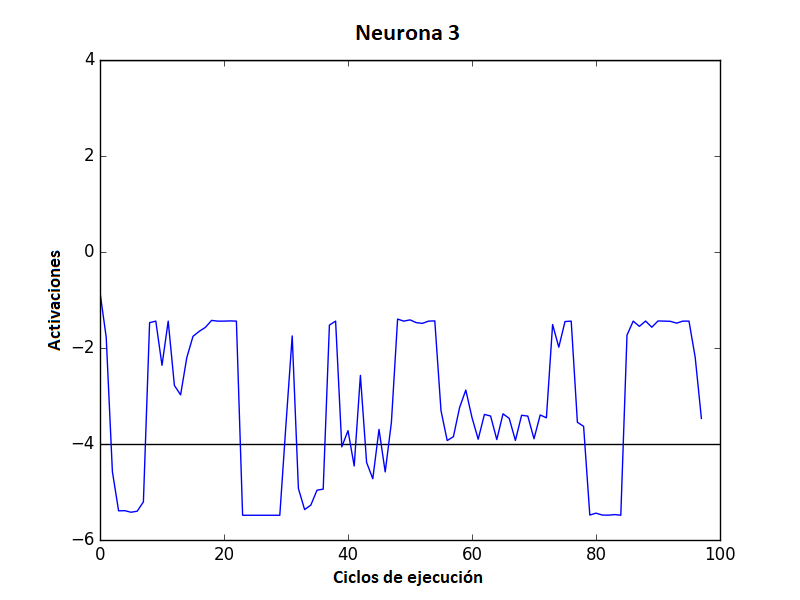
\includegraphics[width=\linewidth]{Imagenes/Agente1Activaciones/Agente3/Neurona2}
\end{subfigure}
\medskip
\begin{subfigure}{0.33\textwidth}
  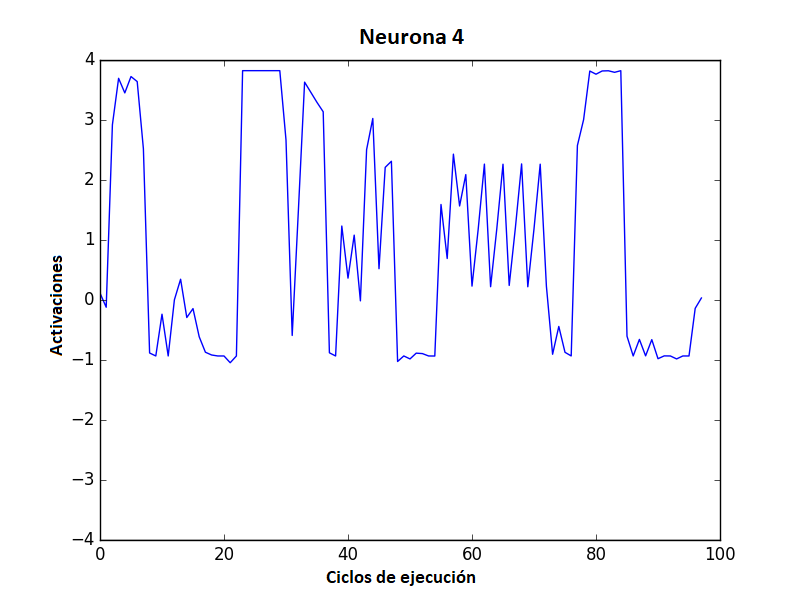
\includegraphics[width=\linewidth]{Imagenes/Agente1Activaciones/Agente3/Neurona3}
\end{subfigure}\hfil % <-- added
\begin{subfigure}{0.33\textwidth}
  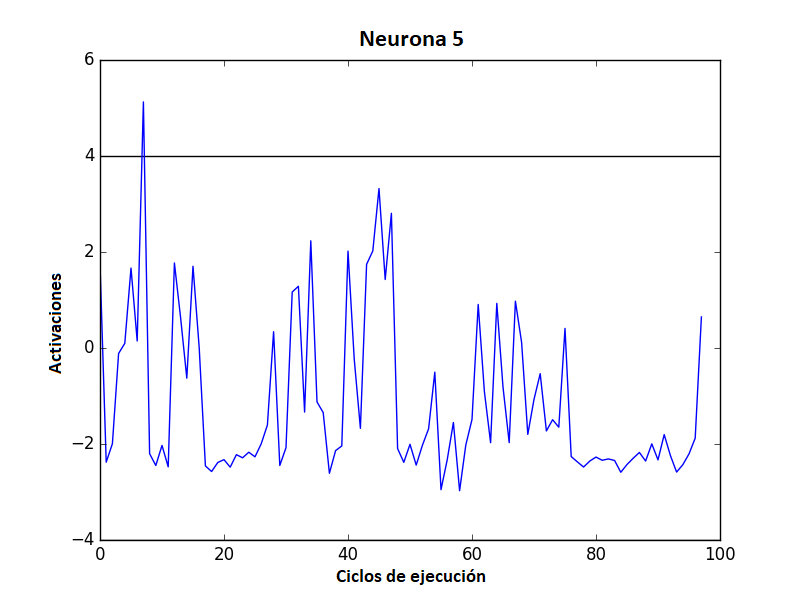
\includegraphics[width=\linewidth]{Imagenes/Agente1Activaciones/Agente3/Neurona4}
\end{subfigure}\hfil % <-- added
\begin{subfigure}{0.33\textwidth}
  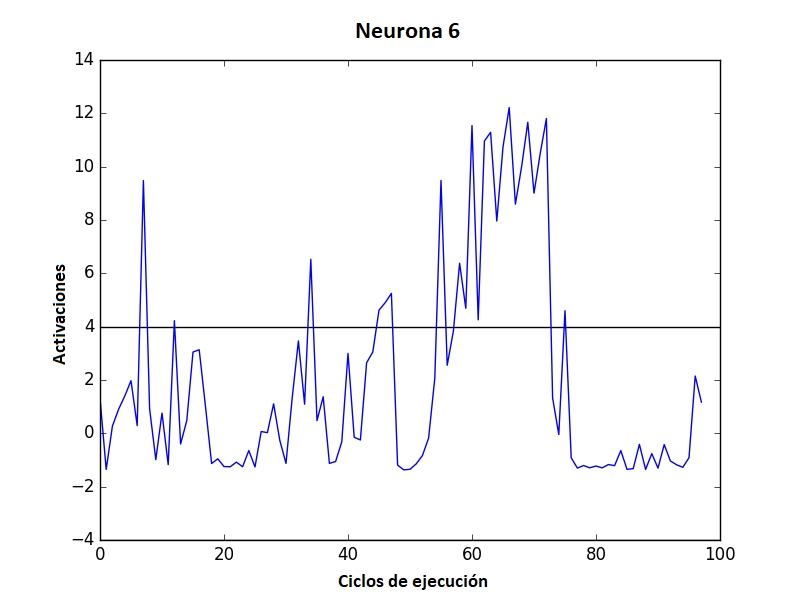
\includegraphics[width=\linewidth]{Imagenes/Agente1Activaciones/Agente3/Neurona5}
\end{subfigure}
\caption{Activaciones de las 6 neuronas del agente número 4 del tipo 1.}
\end{figure}

\begin{figure}[!h]
    \centering % <-- added
\begin{subfigure}{0.33\textwidth}
  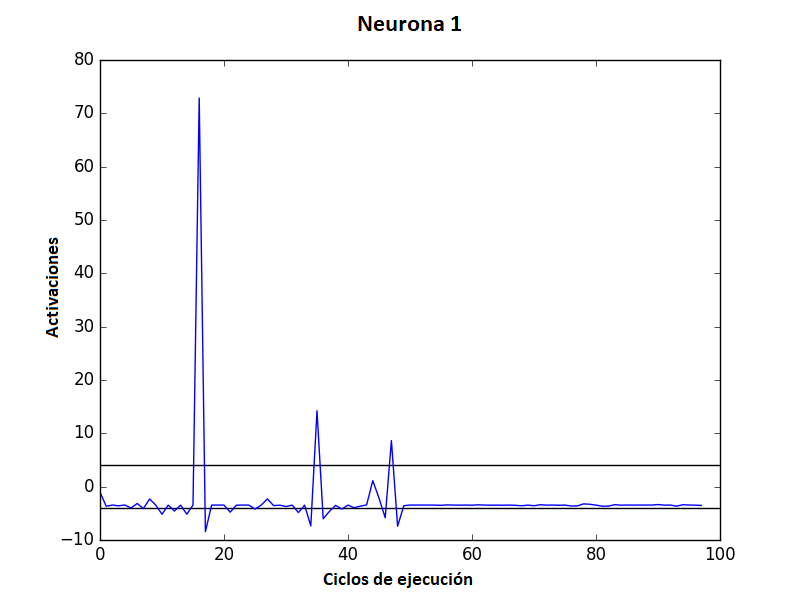
\includegraphics[width=\linewidth]{Imagenes/Agente1Activaciones/Agente4/Neurona0}
\end{subfigure}\hfil % <-- added
\begin{subfigure}{0.33\textwidth}
  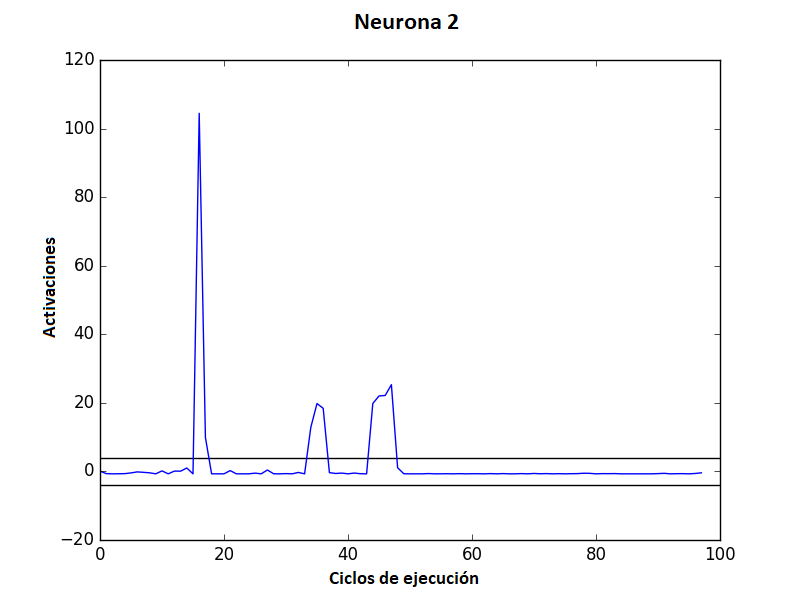
\includegraphics[width=\linewidth]{Imagenes/Agente1Activaciones/Agente4/Neurona1}
\end{subfigure}\hfil % <-- added
\begin{subfigure}{0.33\textwidth}
  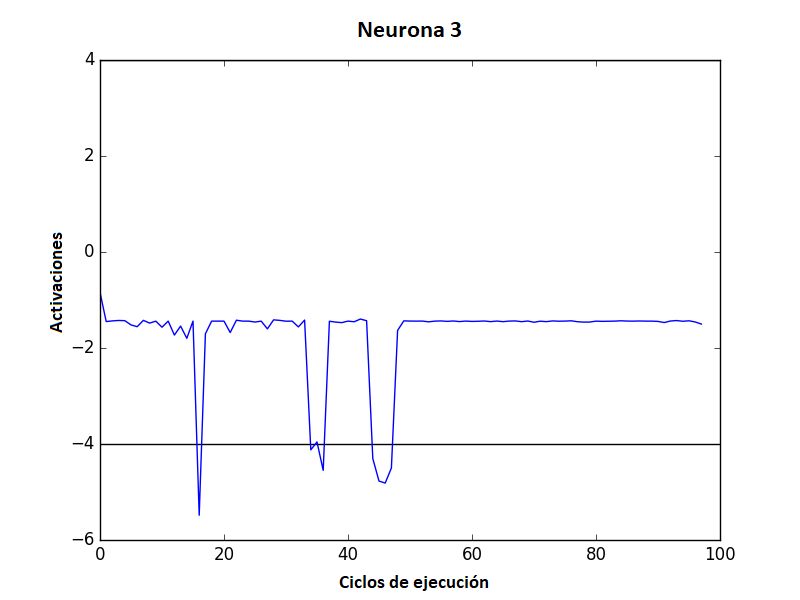
\includegraphics[width=\linewidth]{Imagenes/Agente1Activaciones/Agente4/Neurona2}
\end{subfigure}
\medskip
\begin{subfigure}{0.33\textwidth}
  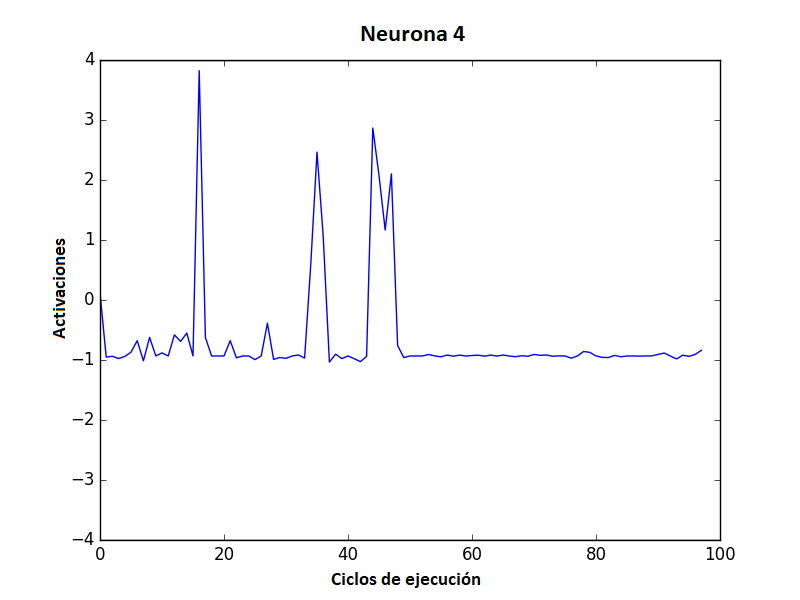
\includegraphics[width=\linewidth]{Imagenes/Agente1Activaciones/Agente4/Neurona3}
\end{subfigure}\hfil % <-- added
\begin{subfigure}{0.33\textwidth}
  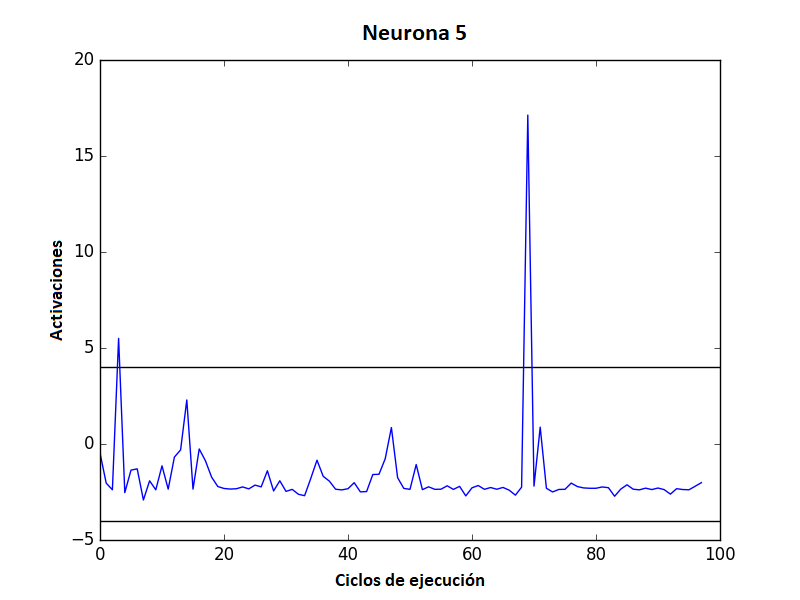
\includegraphics[width=\linewidth]{Imagenes/Agente1Activaciones/Agente4/Neurona4}
\end{subfigure}\hfil % <-- added
\begin{subfigure}{0.33\textwidth}
  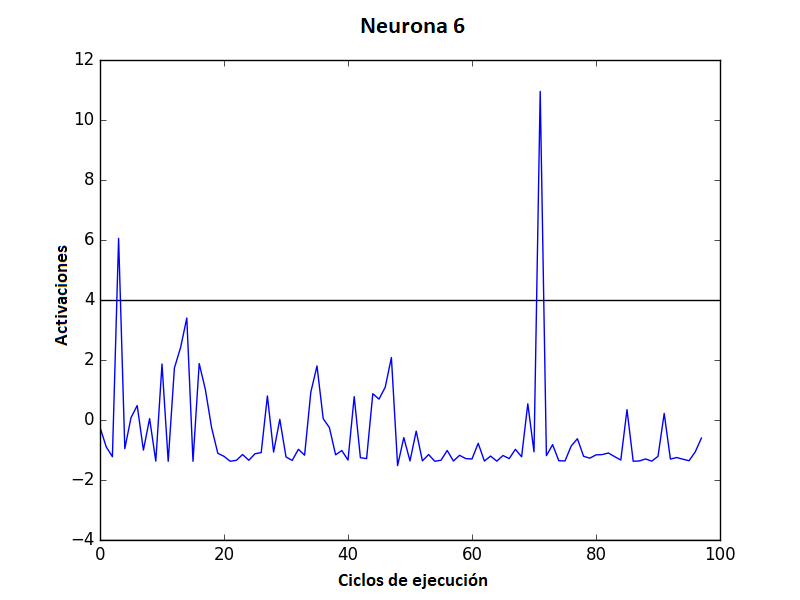
\includegraphics[width=\linewidth]{Imagenes/Agente1Activaciones/Agente4/Neurona5}
\end{subfigure}
\caption{Activaciones de las 6 neuronas del agente número 5 del tipo 1.}
\end{figure}

\chapter{Gráficas completas de las activaciones neuronales del grupo de agentes de tipo 2}\label{ch:anexo4}
\begin{figure}[!h]
    \centering % <-- added
\begin{subfigure}{0.33\textwidth}
  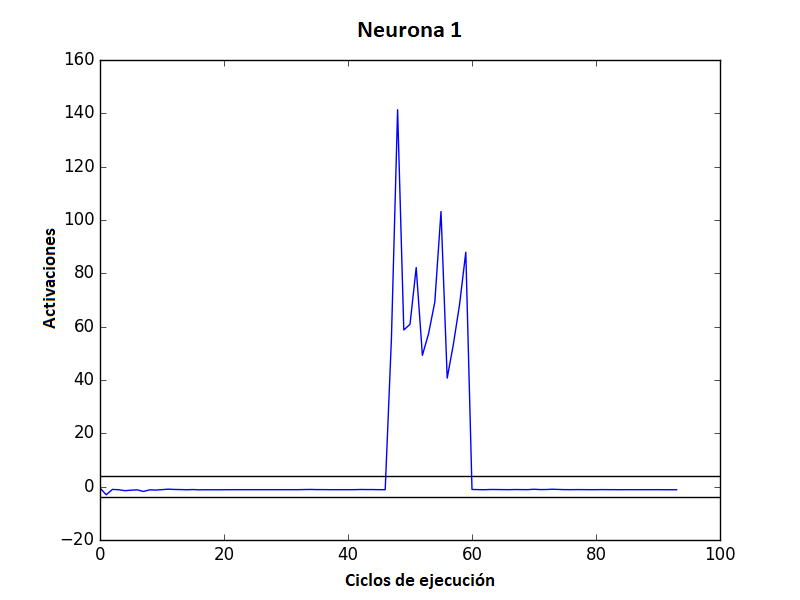
\includegraphics[width=\linewidth]{Imagenes/Agente2Activaciones/Agente0/Neurona0}
\end{subfigure}\hfil % <-- added
\begin{subfigure}{0.33\textwidth}
  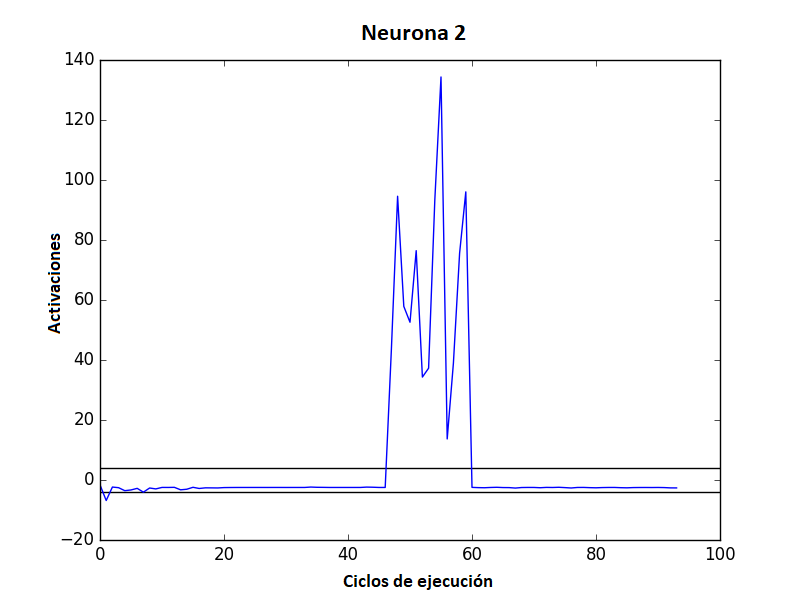
\includegraphics[width=\linewidth]{Imagenes/Agente2Activaciones/Agente0/Neurona1}
\end{subfigure}\hfil % <-- added
\begin{subfigure}{0.33\textwidth}
  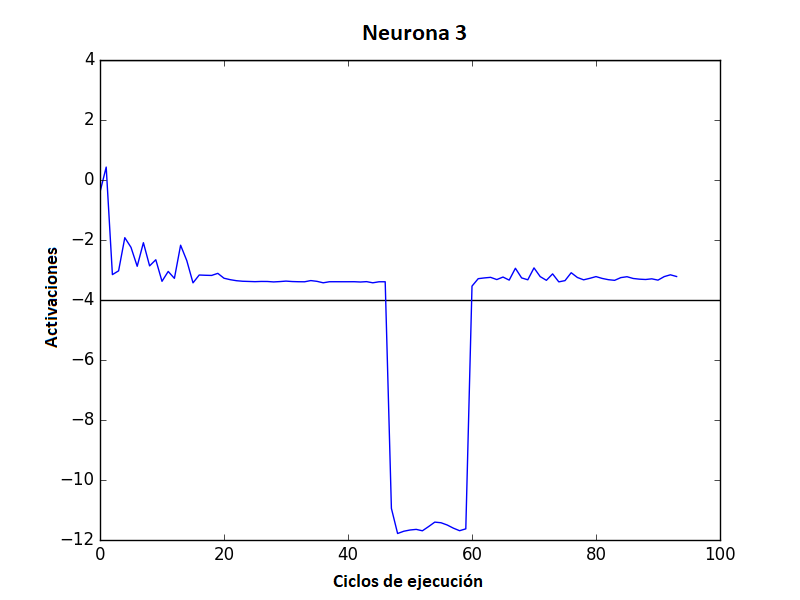
\includegraphics[width=\linewidth]{Imagenes/Agente2Activaciones/Agente0/Neurona2}
\end{subfigure}
\medskip
\begin{subfigure}{0.33\textwidth}
  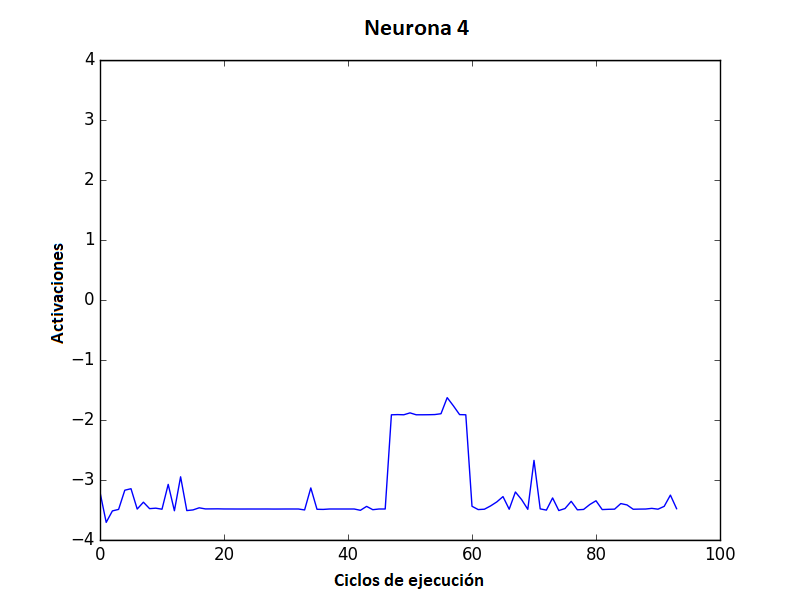
\includegraphics[width=\linewidth]{Imagenes/Agente2Activaciones/Agente0/Neurona3}
\end{subfigure}\hfil % <-- added
\begin{subfigure}{0.33\textwidth}
  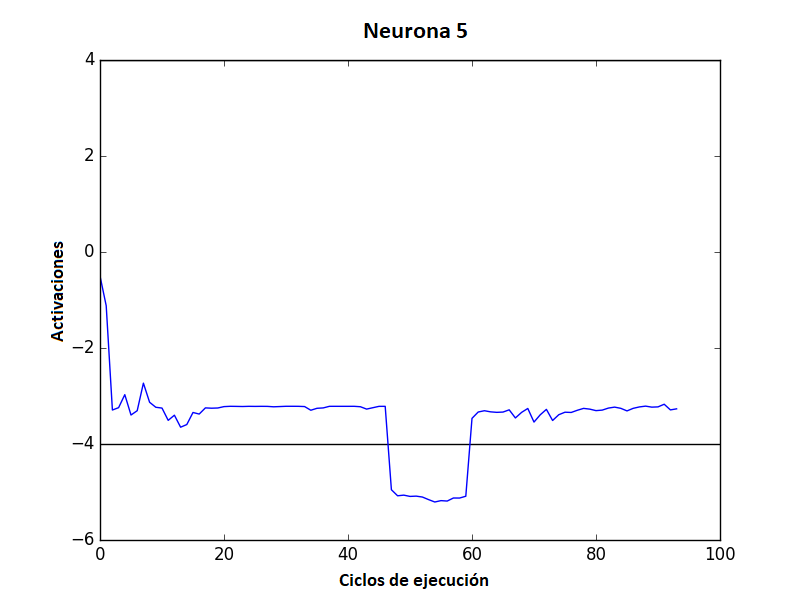
\includegraphics[width=\linewidth]{Imagenes/Agente2Activaciones/Agente0/Neurona4}
\end{subfigure}\hfil % <-- added
\begin{subfigure}{0.33\textwidth}
  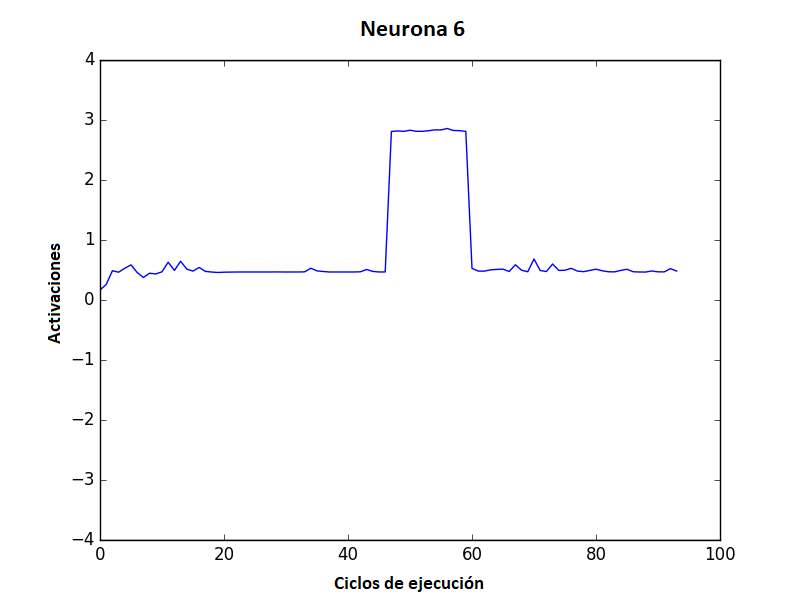
\includegraphics[width=\linewidth]{Imagenes/Agente2Activaciones/Agente0/Neurona5}
\end{subfigure}
\caption{Activaciones de las 6 neuronas del agente número 1 del tipo 2.}
\end{figure}

\begin{figure}[!h]
    \centering % <-- added
\begin{subfigure}{0.33\textwidth}
  \includegraphics[width=\linewidth]{Imagenes/Agente2Activaciones/Agente1/Neurona0}
\end{subfigure}\hfil % <-- added
\begin{subfigure}{0.33\textwidth}
  \includegraphics[width=\linewidth]{Imagenes/Agente2Activaciones/Agente1/Neurona1}
\end{subfigure}\hfil % <-- added
\begin{subfigure}{0.33\textwidth}
  \includegraphics[width=\linewidth]{Imagenes/Agente2Activaciones/Agente1/Neurona2}
\end{subfigure}
\medskip
\begin{subfigure}{0.33\textwidth}
  \includegraphics[width=\linewidth]{Imagenes/Agente2Activaciones/Agente1/Neurona3}
\end{subfigure}\hfil % <-- added
\begin{subfigure}{0.33\textwidth}
  \includegraphics[width=\linewidth]{Imagenes/Agente2Activaciones/Agente1/Neurona4}
\end{subfigure}\hfil % <-- added
\begin{subfigure}{0.33\textwidth}
  \includegraphics[width=\linewidth]{Imagenes/Agente2Activaciones/Agente1/Neurona5}
\end{subfigure}
\caption{Activaciones de las 6 neuronas del agente número 2 del tipo 2.}
\end{figure}

\begin{figure}[!h]
    \centering % <-- added
\begin{subfigure}{0.33\textwidth}
  \includegraphics[width=\linewidth]{Imagenes/Agente2Activaciones/Agente2/Neurona0}
\end{subfigure}\hfil % <-- added
\begin{subfigure}{0.33\textwidth}
  \includegraphics[width=\linewidth]{Imagenes/Agente2Activaciones/Agente2/Neurona1}
\end{subfigure}\hfil % <-- added
\begin{subfigure}{0.33\textwidth}
  \includegraphics[width=\linewidth]{Imagenes/Agente2Activaciones/Agente2/Neurona2}
\end{subfigure}
\medskip
\begin{subfigure}{0.33\textwidth}
  \includegraphics[width=\linewidth]{Imagenes/Agente2Activaciones/Agente2/Neurona3}
\end{subfigure}\hfil % <-- added
\begin{subfigure}{0.33\textwidth}
  \includegraphics[width=\linewidth]{Imagenes/Agente2Activaciones/Agente2/Neurona4}
\end{subfigure}\hfil % <-- added
\begin{subfigure}{0.33\textwidth}
  \includegraphics[width=\linewidth]{Imagenes/Agente2Activaciones/Agente2/Neurona5}
\end{subfigure}
\caption{Activaciones de las 6 neuronas del agente número 3 del tipo 2.}
\end{figure}

\begin{figure}[!h]
    \centering % <-- added
\begin{subfigure}{0.33\textwidth}
  \includegraphics[width=\linewidth]{Imagenes/Agente2Activaciones/Agente3/Neurona0}
\end{subfigure}\hfil % <-- added
\begin{subfigure}{0.33\textwidth}
  \includegraphics[width=\linewidth]{Imagenes/Agente2Activaciones/Agente3/Neurona1}
\end{subfigure}\hfil % <-- added
\begin{subfigure}{0.33\textwidth}
  \includegraphics[width=\linewidth]{Imagenes/Agente2Activaciones/Agente3/Neurona2}
\end{subfigure}
\medskip
\begin{subfigure}{0.33\textwidth}
  \includegraphics[width=\linewidth]{Imagenes/Agente2Activaciones/Agente3/Neurona3}
\end{subfigure}\hfil % <-- added
\begin{subfigure}{0.33\textwidth}
  \includegraphics[width=\linewidth]{Imagenes/Agente2Activaciones/Agente3/Neurona4}
\end{subfigure}\hfil % <-- added
\begin{subfigure}{0.33\textwidth}
  \includegraphics[width=\linewidth]{Imagenes/Agente2Activaciones/Agente3/Neurona5}
\end{subfigure}
\caption{Activaciones de las 6 neuronas del agente número 4 del tipo 2.}
\end{figure}

\begin{figure}[!h]
    \centering % <-- added
\begin{subfigure}{0.33\textwidth}
  \includegraphics[width=\linewidth]{Imagenes/Agente2Activaciones/Agente4/Neurona0}
\end{subfigure}\hfil % <-- added
\begin{subfigure}{0.33\textwidth}
  \includegraphics[width=\linewidth]{Imagenes/Agente2Activaciones/Agente4/Neurona1}
\end{subfigure}\hfil % <-- added
\begin{subfigure}{0.33\textwidth}
  \includegraphics[width=\linewidth]{Imagenes/Agente2Activaciones/Agente4/Neurona2}
\end{subfigure}
\medskip
\begin{subfigure}{0.33\textwidth}
  \includegraphics[width=\linewidth]{Imagenes/Agente2Activaciones/Agente4/Neurona3}
\end{subfigure}\hfil % <-- added
\begin{subfigure}{0.33\textwidth}
  \includegraphics[width=\linewidth]{Imagenes/Agente2Activaciones/Agente4/Neurona4}
\end{subfigure}\hfil % <-- added
\begin{subfigure}{0.33\textwidth}
  \includegraphics[width=\linewidth]{Imagenes/Agente2Activaciones/Agente4/Neurona5}
\end{subfigure}
\caption{Activaciones de las 6 neuronas del agente número 5 del tipo 2.}
\end{figure}

\chapter{Planificación y cronograma}\label{ch:anexo5}
El control de horas del proyecto puede verse representado en la figura \ref{fig:figuraCrono}, donde están indicadas las horas dedicadas a cada tarea del proyecto cada semana de la duración del mismo. Cabe aclarar que no se ha llevado control de horas de la tarea
``investigación y lectura de documentación'' ya que ha sido una tarea presente durante toda la duración del proyecto.
\begin{figure}[H]
  \centering
  \includegraphics[width=1.0\textwidth]{Imagenes/Cronograma}
	\caption{Cronograma del proyecto dividido por semanas, incluyendo las horas dedicadas cada semana a cada tarea.}
	\label{fig:figuraCrono}
\end{figure}

En total se han invertido 417 horas a la realización de este Trabajo de Fin de Grado.



%%%%%%%%%%%%%%%%%%%%%%%%%%%%%%%%%%%%%%%%%%%%%%%%%%%%%%%%%%%%%%%%%%%%%%%%%%%%%%%%%%%


\end{document}
